\chapter{Implementing Motors in Rigid Multibody Algorithms}
\label{chp:contrib_ABA}

This chapter describes the formalism and the algorithms involved in the conditioning of multibody systems behavior, taking into account motor dynamics in the framework of recursive computation methods. In particular, in the first part, the problem of considering rotor dynamics is addressed by modifying the inertia matrix of the system and introducing a new term in the Coriolis vector. This approach will be referred to as \textit{Inertia-Matrix Method}. While being relatively simple to implement, this method forces some hypotheses that can limit its range of application. An alternative approach is described in the second part of the chapter, in which the process of injecting the motor parameters in the Articulated Body Algorithm (\ac{ABA}) is discussed. In the last section, a comparison between the two approaches is presented, in order to highlight the potentialities and the drawbacks of each method.

\section{Rotor-conditioned Forward Dynamics with Inertia-Matrix Method}

\begin{figure}
    \centering
    \caption{Harmonic Drive Model}
    \label{fig:harmonic_drive}
    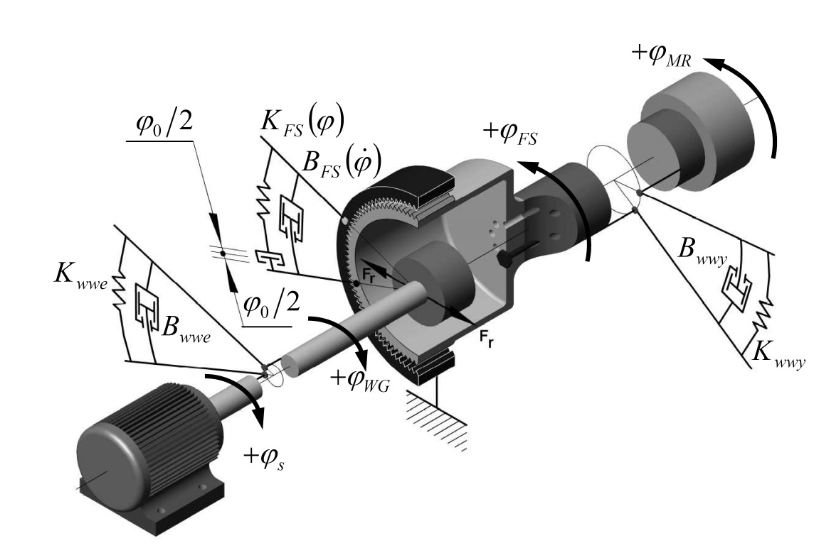
\includegraphics[width=0.7\textwidth]{Images/harmonic_drive.png}
\end{figure}

Starting from the equation of motion of a robot manipulator, as expressed in \cref{sec:back_eom}:

\begin{equation}
    \mathbb{M}(q)\dot{\boldsymbol{\nu}} + \mathbf{h}(q,\boldsymbol{\nu}) = \mathbf{B}\boldsymbol{\tau} + \mathbf{J} ^\top \mathbf{f}
\end{equation}

where $\mathbb{M}(q)$ is the inertia matrix, $\mathbf{h}(q,\boldsymbol{\nu})$ is the Coriolis vector, $\mathbf{B}$ is the selection matrix for the actuation torques, $\boldsymbol{\tau}$ is actuation torques vector, $\mathbf{J}$ is the Jacobian matrix and $\mathbf{f}$ is the external forces vector, we can isolate the terms related to the base link from the rest of the kinematic chain:

\begin{align}
    \boldsymbol{\nu} =
    \begin{bmatrix}
        \mathrm{\mathbf{v}} \\
        \dot{\mathbf{s}}
    \end{bmatrix} &  &
    \dot{\boldsymbol{\nu}} =
    \begin{bmatrix}
        \dot{\mathrm{\mathbf{v}}} \\
        \ddot{\mathbf{s}}
    \end{bmatrix}
\end{align}

where $\mathrm{\mathbf{v}} \in \mathrm{SO}(3)$ and $\mathbf{s} \in \mathbb{R}^{n}$. Therefore, the equation of motion can be rewritten in its matrix form as:

\begin{equation}
    \begin{bmatrix}
        \mathbb{M} _{\mathcal{B}}(q)        & \mathbb{M} _{\mathcal{B}S}(q) \\
        \mathbb{M} _{\mathcal{B}S} ^\top(q) & \mathbb{M} _s(q)
    \end{bmatrix}
    \begin{bmatrix}
        \dot{\mathrm{\mathbf{v}}} \\
        \ddot{\mathbf{s}}
    \end{bmatrix}+
    \begin{bmatrix}
        \mathbf{h} _{\mathcal{B}} \\
        \mathbf{h} _S
    \end{bmatrix}=
    \begin{bmatrix}
        \mathbbm{0} \\
        \mathbbm{1}
    \end{bmatrix}
    \boldsymbol{\tau}
    +
    \begin{bmatrix}
        \mathbf{J} _{\mathcal{B}} \\
        \mathbf{J} _S
    \end{bmatrix} ^\top
    \mathbf{f}
\end{equation}

Given that the dynamics of the set of $N _M = n$ motors can be described by \cref{eqn:mot_dyn} and graphically represented as in \cref{fig:harmonic_drive} \citep{folga2010}, we can rewrite the equation of motion as:

\begin{equation}
    \mathbb{M} ^M \ddot{\boldsymbol{\theta}} + \mathbf{K}_v \dot{\boldsymbol{\theta}} = \boldsymbol{\tau}_m
    \label{eqn:mot_dyn}
\end{equation}

where $\mathbf{K}_v \in \mathbb{R}^n$ is the diagonal matrix of motor viscous friction coefficients and $\mathbb{M}^M \in \mathbb{R}^{n \times n}$ is the matrix of motors' inertias. Considering that given the set of transmission ratios $\boldsymbol{\Gamma} \in \mathbb{R}^n$, the relation between the joints' velocities and the motors' velocities is:

\begin{align}
    \mathbf{s} = \boldsymbol{\theta} \boldsymbol{\Gamma} &  & \dot{\mathbf{s}} = \frac{d}{dt} \mathbf{s} = \dot{\boldsymbol{\theta}} \boldsymbol{\Gamma} &  & \ddot{\mathbf{s}} = \frac{d^2}{dt^2} \mathbf{s} = \ddot{\boldsymbol{\theta}} \boldsymbol{\Gamma}
\end{align}

we can rewrite the equation \cref{eqn:mot_dyn} in the joints' space as:

\begin{equation}
    \label{eqn:mot_dyn_jointspace}
    \boldsymbol{\tau} = \boldsymbol{\Gamma} ^{-T} (\mathbb{M} ^M\boldsymbol{\Gamma} ^{-1} \ddot{s} + \mathbf{K}_v \boldsymbol{\Gamma} ^{-1}\dot{s})
\end{equation}

Therefore, the \ac{EoM} of the multibody system can be reformulated as:

\begin{equation}
    \underbrace{\begin{bmatrix}
            \mathbb{M} _{\mathcal{B}}(q)        & \mathbb{M} _{\mathcal{B}S}(q)                                                      \\
            \mathbb{M} _{\mathcal{B}S} ^\top(q) & \mathbb{M} _s(q) + \boldsymbol{\Gamma} ^{-T}\mathbb{M} ^M\boldsymbol{\Gamma} ^{-1}
        \end{bmatrix}} _{\mathbf{\bar{M}}(q)}
    \begin{bmatrix}
        \dot{\mathrm{\mathbf{v}}} \\
        \ddot{\mathbf{s}}
    \end{bmatrix}+
    \mathbf{h}
    (q,\boldsymbol{\nu}) =
    \underbrace{\begin{bmatrix}
            \mathbbm{0} \\
            \boldsymbol{\Gamma} ^{-T}
        \end{bmatrix}} _{\mathbf{\bar{B}}}
    \boldsymbol{\tau} _m
    +
    \mathbf{J} ^\top
    \mathbf{f}
    -
    \underbrace{\begin{bmatrix}
            \mathbbm{0} \\
            \boldsymbol{\Gamma} ^{-T}\mathbf{K _v}\boldsymbol{\Gamma} ^{-1}
        \end{bmatrix}} _\mathbf{\bar{K _v}}
    \begin{bmatrix}
        \mathrm{\mathbf{v}} \\
        \dot{\mathbf{s}}
    \end{bmatrix}
\end{equation}

only under the following hypotheses:

\begin{enumerate}
    \item The motors are rigidly attached to the links by the transmission;
    \item The axis of rotation of the motors is aligned with the axis of rotation of the joints;
    \item The gearbox inertia is negligible compared to the link inertia;
    \item The couplings do not introduce any additional friction:
    \item The internal motor friction is modelled as viscous friction only;
    \item The \ac{CoM} of the motor is coincident with its axis of rotation, e.g. the angular momentum of the motor is only due to its spinning motion.
\end{enumerate}

In a more compact form, the \ac{EoM} can be also expressed as:

\begin{equation}
    \mathbf{\bar{M}}(q)\dot{\boldsymbol{\nu}} + \mathbf{h}(q,\boldsymbol{\nu}) = \mathbf{\bar{B}}\boldsymbol{\tau} _m + \mathbf{J} ^\top \mathbf{f} - \bar{\mathbf{K _v}}\boldsymbol{\nu}
\end{equation}

which yields the acceleration of the system:

\begin{equation}
    \dot{\boldsymbol{\nu}} = \mathbf{\bar{M}}(q) ^{-1} (\mathbf{\bar{B}}\boldsymbol{\tau} _m + \mathbf{J} ^\top \mathbf{f} - \mathbf{h}(q,\boldsymbol{\nu}) - \bar{\mathbf{K _v}}\boldsymbol{\nu})
\end{equation}

\section{ABA with Motor Dynamics}

In \cref{subsec:back_aba} we briefly introduced the recursive relations of the \ac{ABA} algorithm. In this section, we will describe how to modify the algorithm in order to take into account the motor dynamics. The main idea is to consider the rotor as an additional link in the kinematic chain, and to modify the inertia matrix and the Coriolis vector accordingly. In particular, we can summarizes the hypotheses behind this approach as follows:

\begin{enumerate}
    \item the gearbox inertia is negligible compared to the link inertia;
    \item the motion subspace of the rotor is the same as the motion subspace of the link to which it is attached scaled by the gear ratio, e.g. the free modes of the rotor are the same as the free modes of the link to which it is attached:
    \item The couplings do not introduce any additional friction
    \item The internal motor friction is modelled as viscous friction only;
    \item The \ac{CoM} of the motor is coincident with its axis of rotation, e.g. the angular momentum of the motor is only due to its spinning motion.
\end{enumerate}

With these hypotheses, we can reformulate the motion subspace of the rotor attached to joint $i$ as:

\begin{equation}
    \label{eqn:motor_subspace}
    {} ^M \boldsymbol{\Phi} _i = \boldsymbol{\Gamma} _i \boldsymbol{\Phi} _i
\end{equation}


% === FIG: Unconstrained Tree === %
\begin{figure}
    \centering
    \caption{Visual comparison between the unconstrained and constrained kinematic tree.}
    \label{fig:uc_and_constr_tree}
    \subfloat[Constrained System]{
        \resizebox{0.45\textwidth}{!}{
            \tikzset {_djnj2rsc4/.code = {\pgfsetadditionalshadetransform{ \pgftransformshift{\pgfpoint{0 bp } { 0 bp }  }  \pgftransformrotate{-117 }  \pgftransformscale{2 }  }}}
\pgfdeclarehorizontalshading{_idu07h52c}{150bp}{rgb(0bp)=(1,1,1);
    rgb(37.5bp)=(1,1,1);
    rgb(50.08184160505022bp)=(0.95,0.95,0.95);
    rgb(57.64583042689732bp)=(0.88,0.88,0.88);
    rgb(61.33184160505022bp)=(0.96,0.96,0.96);
    rgb(100bp)=(0.96,0.96,0.96)}
\tikzset {_jsyk5ax1n/.code = {\pgfsetadditionalshadetransform{ \pgftransformshift{\pgfpoint{0 bp } { 0 bp }  }  \pgftransformrotate{-117 }  \pgftransformscale{2 }  }}}
\pgfdeclarehorizontalshading{_92edxt770}{150bp}{rgb(0bp)=(1,1,1);
    rgb(37.5bp)=(1,1,1);
    rgb(50.08184160505022bp)=(0.95,0.95,0.95);
    rgb(57.64583042689732bp)=(0.88,0.88,0.88);
    rgb(61.33184160505022bp)=(0.96,0.96,0.96);
    rgb(100bp)=(0.96,0.96,0.96)}
\tikzset {_b0gplq11g/.code = {\pgfsetadditionalshadetransform{ \pgftransformshift{\pgfpoint{0 bp } { 0 bp }  }  \pgftransformrotate{-117 }  \pgftransformscale{2 }  }}}
\pgfdeclarehorizontalshading{_x22po1g8w}{150bp}{rgb(0bp)=(1,1,1);
    rgb(37.5bp)=(1,1,1);
    rgb(50.08184160505022bp)=(0.95,0.95,0.95);
    rgb(57.64583042689732bp)=(0.88,0.88,0.88);
    rgb(61.33184160505022bp)=(0.96,0.96,0.96);
    rgb(100bp)=(0.96,0.96,0.96)}
\tikzset {_ivsfd2s3h/.code = {\pgfsetadditionalshadetransform{ \pgftransformshift{\pgfpoint{0 bp } { 0 bp }  }  \pgftransformrotate{-117 }  \pgftransformscale{2 }  }}}
\pgfdeclarehorizontalshading{_8u84rjokz}{150bp}{rgb(0bp)=(1,1,1);
    rgb(37.5bp)=(1,1,1);
    rgb(50.08184160505022bp)=(0.95,0.95,0.95);
    rgb(57.64583042689732bp)=(0.88,0.88,0.88);
    rgb(61.33184160505022bp)=(0.96,0.96,0.96);
    rgb(100bp)=(0.96,0.96,0.96)}
\tikzset {_5pcd2h8hv/.code = {\pgfsetadditionalshadetransform{ \pgftransformshift{\pgfpoint{0 bp } { 0 bp }  }  \pgftransformrotate{-117 }  \pgftransformscale{2 }  }}}
\pgfdeclarehorizontalshading{_lvec74ltu}{150bp}{rgb(0bp)=(1,1,1);
    rgb(37.5bp)=(1,1,1);
    rgb(50.08184160505022bp)=(0.95,0.95,0.95);
    rgb(57.64583042689732bp)=(0.88,0.88,0.88);
    rgb(61.33184160505022bp)=(0.96,0.96,0.96);
    rgb(100bp)=(0.96,0.96,0.96)}
\tikzset {_37uba45qs/.code = {\pgfsetadditionalshadetransform{ \pgftransformshift{\pgfpoint{0 bp } { 0 bp }  }  \pgftransformrotate{-117 }  \pgftransformscale{2 }  }}}
\pgfdeclarehorizontalshading{_ik4ni4me2}{150bp}{rgb(0bp)=(1,1,1);
    rgb(37.5bp)=(1,1,1);
    rgb(50.08184160505022bp)=(0.95,0.95,0.95);
    rgb(57.64583042689732bp)=(0.88,0.88,0.88);
    rgb(61.33184160505022bp)=(0.96,0.96,0.96);
    rgb(100bp)=(0.96,0.96,0.96)}
\tikzset {_z01vd74d5/.code = {\pgfsetadditionalshadetransform{ \pgftransformshift{\pgfpoint{0 bp } { 0 bp }  }  \pgftransformrotate{-117 }  \pgftransformscale{2 }  }}}
\pgfdeclarehorizontalshading{_rhf2dk4cx}{150bp}{rgb(0bp)=(1,1,1);
    rgb(37.5bp)=(1,1,1);
    rgb(50.08184160505022bp)=(0.95,0.95,0.95);
    rgb(57.64583042689732bp)=(0.88,0.88,0.88);
    rgb(61.33184160505022bp)=(0.96,0.96,0.96);
    rgb(100bp)=(0.96,0.96,0.96)}
\tikzset {_9fj7ssnk1/.code = {\pgfsetadditionalshadetransform{ \pgftransformshift{\pgfpoint{0 bp } { 0 bp }  }  \pgftransformrotate{-117 }  \pgftransformscale{2 }  }}}
\pgfdeclarehorizontalshading{_nn6marsz8}{150bp}{rgb(0bp)=(1,1,1);
    rgb(37.5bp)=(1,1,1);
    rgb(50.08184160505022bp)=(0.95,0.95,0.95);
    rgb(57.64583042689732bp)=(0.88,0.88,0.88);
    rgb(61.33184160505022bp)=(0.96,0.96,0.96);
    rgb(100bp)=(0.96,0.96,0.96)}
\tikzset {_vxd4nfhmk/.code = {\pgfsetadditionalshadetransform{ \pgftransformshift{\pgfpoint{0 bp } { 0 bp }  }  \pgftransformrotate{-117 }  \pgftransformscale{2 }  }}}
\pgfdeclarehorizontalshading{_be3tjpf6d}{150bp}{rgb(0bp)=(1,1,1);
    rgb(37.5bp)=(1,1,1);
    rgb(50.08184160505022bp)=(0.95,0.95,0.95);
    rgb(57.64583042689732bp)=(0.88,0.88,0.88);
    rgb(61.33184160505022bp)=(0.96,0.96,0.96);
    rgb(100bp)=(0.96,0.96,0.96)}
\tikzset {_syya3oz6t/.code = {\pgfsetadditionalshadetransform{ \pgftransformshift{\pgfpoint{0 bp } { 0 bp }  }  \pgftransformrotate{-117 }  \pgftransformscale{2 }  }}}
\pgfdeclarehorizontalshading{_73496xns5}{150bp}{rgb(0bp)=(1,1,1);
    rgb(37.5bp)=(1,1,1);
    rgb(50.08184160505022bp)=(0.95,0.95,0.95);
    rgb(57.64583042689732bp)=(0.88,0.88,0.88);
    rgb(61.33184160505022bp)=(0.96,0.96,0.96);
    rgb(100bp)=(0.96,0.96,0.96)}
\tikzset{every picture/.style={line width=0.75pt}}
\begin{tikzpicture}[x=0.75pt,y=0.75pt,yscale=-1,xscale=1]
    \path  [shading=_idu07h52c,_djnj2rsc4] (360.92,117.33) .. controls (360.92,108.96) and (384.78,102.17) .. (414.21,102.17) .. controls (443.64,102.17) and (467.5,108.96) .. (467.5,117.33) .. controls (467.5,125.71) and (443.64,132.5) .. (414.21,132.5) .. controls (384.78,132.5) and (360.92,125.71) .. (360.92,117.33) -- cycle ;
    \draw  [color={rgb, 255:red, 0; green, 0; blue, 0 }  ,draw opacity=1 ][line width=0.75]  (360.92,117.33) .. controls (360.92,108.96) and (384.78,102.17) .. (414.21,102.17) .. controls (443.64,102.17) and (467.5,108.96) .. (467.5,117.33) .. controls (467.5,125.71) and (443.64,132.5) .. (414.21,132.5) .. controls (384.78,132.5) and (360.92,125.71) .. (360.92,117.33) -- cycle ;
    \path  [shading=_92edxt770,_jsyk5ax1n] (548.22,34.11) .. controls (554.45,39.72) and (543.53,61.99) .. (523.84,83.87) .. controls (504.15,105.75) and (483.14,118.94) .. (476.92,113.33) .. controls (470.69,107.73) and (481.61,85.45) .. (501.3,63.58) .. controls (520.99,41.7) and (542,28.51) .. (548.22,34.11) -- cycle ;
    \draw  [color={rgb, 255:red, 0; green, 0; blue, 0 }  ,draw opacity=1 ][line width=0.75]  (548.22,34.11) .. controls (554.45,39.72) and (543.53,61.99) .. (523.84,83.87) .. controls (504.15,105.75) and (483.14,118.94) .. (476.92,113.33) .. controls (470.69,107.73) and (481.61,85.45) .. (501.3,63.58) .. controls (520.99,41.7) and (542,28.51) .. (548.22,34.11) -- cycle ;
    \path  [shading=_x22po1g8w,_b0gplq11g] (467.5,117.33) .. controls (467.5,114.46) and (469.83,112.13) .. (472.71,112.13) .. controls (475.58,112.13) and (477.92,114.46) .. (477.92,117.33) .. controls (477.92,120.21) and (475.58,122.54) .. (472.71,122.54) .. controls (469.83,122.54) and (467.5,120.21) .. (467.5,117.33) -- cycle ;
    \draw  [color={rgb, 255:red, 0; green, 0; blue, 0 }  ,draw opacity=1 ][line width=0.75]  (467.5,117.33) .. controls (467.5,114.46) and (469.83,112.13) .. (472.71,112.13) .. controls (475.58,112.13) and (477.92,114.46) .. (477.92,117.33) .. controls (477.92,120.21) and (475.58,122.54) .. (472.71,122.54) .. controls (469.83,122.54) and (467.5,120.21) .. (467.5,117.33) -- cycle ;
    \path  [shading=_8u84rjokz,_ivsfd2s3h] (352.22,121.61) .. controls (358.45,127.22) and (347.53,149.49) .. (327.84,171.37) .. controls (308.15,193.25) and (287.14,206.44) .. (280.92,200.83) .. controls (274.69,195.23) and (285.61,172.95) .. (305.3,151.08) .. controls (324.99,129.2) and (346,116.01) .. (352.22,121.61) -- cycle ;
    \draw  [color={rgb, 255:red, 0; green, 0; blue, 0 }  ,draw opacity=1 ][line width=0.75]  (352.22,121.61) .. controls (358.45,127.22) and (347.53,149.49) .. (327.84,171.37) .. controls (308.15,193.25) and (287.14,206.44) .. (280.92,200.83) .. controls (274.69,195.23) and (285.61,172.95) .. (305.3,151.08) .. controls (324.99,129.2) and (346,116.01) .. (352.22,121.61) -- cycle ;
    \path  [shading=_lvec74ltu,_5pcd2h8hv] (350.5,117.33) .. controls (350.5,114.46) and (352.83,112.13) .. (355.71,112.13) .. controls (358.58,112.13) and (360.92,114.46) .. (360.92,117.33) .. controls (360.92,120.21) and (358.58,122.54) .. (355.71,122.54) .. controls (352.83,122.54) and (350.5,120.21) .. (350.5,117.33) -- cycle ;
    \draw  [color={rgb, 255:red, 0; green, 0; blue, 0 }  ,draw opacity=1 ][line width=0.75]  (350.5,117.33) .. controls (350.5,114.46) and (352.83,112.13) .. (355.71,112.13) .. controls (358.58,112.13) and (360.92,114.46) .. (360.92,117.33) .. controls (360.92,120.21) and (358.58,122.54) .. (355.71,122.54) .. controls (352.83,122.54) and (350.5,120.21) .. (350.5,117.33) -- cycle ;
    \path  [shading=_ik4ni4me2,_37uba45qs] (272.46,204.96) .. controls (272.46,202.08) and (274.79,199.75) .. (277.67,199.75) .. controls (280.54,199.75) and (282.87,202.08) .. (282.87,204.96) .. controls (282.87,207.83) and (280.54,210.17) .. (277.67,210.17) .. controls (274.79,210.17) and (272.46,207.83) .. (272.46,204.96) -- cycle ;
    \draw  [color={rgb, 255:red, 0; green, 0; blue, 0 }  ,draw opacity=1 ][line width=0.75]  (272.46,204.96) .. controls (272.46,202.08) and (274.79,199.75) .. (277.67,199.75) .. controls (280.54,199.75) and (282.87,202.08) .. (282.87,204.96) .. controls (282.87,207.83) and (280.54,210.17) .. (277.67,210.17) .. controls (274.79,210.17) and (272.46,207.83) .. (272.46,204.96) -- cycle ;
    \path  [shading=_rhf2dk4cx,_z01vd74d5] (170.95,143.93) .. controls (163.63,148.01) and (146.08,130.48) .. (131.74,104.78) .. controls (117.4,79.08) and (111.7,54.93) .. (119.02,50.85) .. controls (126.33,46.77) and (143.89,64.3) .. (158.23,90) .. controls (172.57,115.7) and (178.26,139.85) .. (170.95,143.93) -- cycle ;
    \draw  [color={rgb, 255:red, 0; green, 0; blue, 0 }  ,draw opacity=1 ][line width=0.75]  (170.95,143.93) .. controls (163.63,148.01) and (146.08,130.48) .. (131.74,104.78) .. controls (117.4,79.08) and (111.7,54.93) .. (119.02,50.85) .. controls (126.33,46.77) and (143.89,64.3) .. (158.23,90) .. controls (172.57,115.7) and (178.26,139.85) .. (170.95,143.93) -- cycle ;
    \path  [shading=_nn6marsz8,_9fj7ssnk1] (179.33,150.95) .. controls (183.31,143.58) and (207.53,148.94) .. (233.43,162.93) .. controls (259.32,176.91) and (277.09,194.22) .. (273.11,201.59) .. controls (269.13,208.96) and (244.91,203.6) .. (219.01,189.62) .. controls (193.12,175.63) and (175.35,158.32) .. (179.33,150.95) -- cycle ;
    \draw  [color={rgb, 255:red, 0; green, 0; blue, 0 }  ,draw opacity=1 ][line width=0.75]  (179.33,150.95) .. controls (183.31,143.58) and (207.53,148.94) .. (233.43,162.93) .. controls (259.32,176.91) and (277.09,194.22) .. (273.11,201.59) .. controls (269.13,208.96) and (244.91,203.6) .. (219.01,189.62) .. controls (193.12,175.63) and (175.35,158.32) .. (179.33,150.95) -- cycle ;
    \path  [shading=_be3tjpf6d,_vxd4nfhmk] (174.79,153.61) .. controls (171.92,153.71) and (169.51,151.45) .. (169.42,148.58) .. controls (169.32,145.7) and (171.58,143.3) .. (174.45,143.2) .. controls (177.33,143.11) and (179.73,145.36) .. (179.83,148.24) .. controls (179.92,151.11) and (177.67,153.52) .. (174.79,153.61) -- cycle ;
    \draw  [color={rgb, 255:red, 0; green, 0; blue, 0 }  ,draw opacity=1 ][line width=0.75]  (174.79,153.61) .. controls (171.92,153.71) and (169.51,151.45) .. (169.42,148.58) .. controls (169.32,145.7) and (171.58,143.3) .. (174.45,143.2) .. controls (177.33,143.11) and (179.73,145.36) .. (179.83,148.24) .. controls (179.92,151.11) and (177.67,153.52) .. (174.79,153.61) -- cycle ;
    \path  [shading=_73496xns5,_syya3oz6t] (540.88,206.7) .. controls (534.23,211.8) and (514.33,196.98) .. (496.44,173.61) .. controls (478.55,150.24) and (469.43,127.17) .. (476.09,122.08) .. controls (482.74,116.98) and (502.63,131.8) .. (520.53,155.17) .. controls (538.42,178.54) and (547.53,201.61) .. (540.88,206.7) -- cycle ;
    \draw  [color={rgb, 255:red, 0; green, 0; blue, 0 }  ,draw opacity=1 ][line width=0.75]  (540.88,206.7) .. controls (534.23,211.8) and (514.33,196.98) .. (496.44,173.61) .. controls (478.55,150.24) and (469.43,127.17) .. (476.09,122.08) .. controls (482.74,116.98) and (502.63,131.8) .. (520.53,155.17) .. controls (538.42,178.54) and (547.53,201.61) .. (540.88,206.7) -- cycle ;
    \draw [color={rgb, 255:red, 74; green, 144; blue, 226 }  ,draw opacity=1 ]   (103.21,151.6) -- (172.62,148.5) ;
    \draw [shift={(174.62,148.41)}, rotate = 177.44] [fill={rgb, 255:red, 74; green, 144; blue, 226 }  ,fill opacity=1 ][line width=0.08]  [draw opacity=0] (12,-3) -- (0,0) -- (12,3) -- cycle    ;
    \draw [color={rgb, 255:red, 74; green, 144; blue, 226 }  ,draw opacity=1 ]   (373.78,57.81) -- (356.29,115.42) ;
    \draw [shift={(355.71,117.33)}, rotate = 286.89] [fill={rgb, 255:red, 74; green, 144; blue, 226 }  ,fill opacity=1 ][line width=0.08]  [draw opacity=0] (12,-3) -- (0,0) -- (12,3) -- cycle    ;
    \draw [color={rgb, 255:red, 74; green, 144; blue, 226 }  ,draw opacity=1 ]   (465.03,205.67) -- (534.45,202.56) ;
    \draw [shift={(536.44,202.47)}, rotate = 177.44] [fill={rgb, 255:red, 74; green, 144; blue, 226 }  ,fill opacity=1 ][line width=0.08]  [draw opacity=0] (12,-3) -- (0,0) -- (12,3) -- cycle    ;
    \draw [color={rgb, 255:red, 74; green, 144; blue, 226 }  ,draw opacity=1 ]   (492.37,61.67) -- (473.37,115.45) ;
    \draw [shift={(472.71,117.33)}, rotate = 289.46] [fill={rgb, 255:red, 74; green, 144; blue, 226 }  ,fill opacity=1 ][line width=0.08]  [draw opacity=0] (12,-3) -- (0,0) -- (12,3) -- cycle    ;
    \draw  [draw opacity=0] (179.21,161.74) .. controls (177.77,162.22) and (176.23,162.48) .. (174.62,162.48) .. controls (166.68,162.48) and (160.25,156.18) .. (160.25,148.41) .. controls (160.25,140.64) and (166.68,134.34) .. (174.62,134.34) .. controls (182.56,134.34) and (189,140.64) .. (189,148.41) .. controls (189,150) and (188.73,151.53) .. (188.23,152.95) -- (174.62,148.41) -- cycle ; \draw [color={rgb, 255:red, 74; green, 144; blue, 226 }  ,draw opacity=1 ]   (179.21,161.74) .. controls (177.77,162.22) and (176.23,162.48) .. (174.62,162.48) .. controls (166.68,162.48) and (160.25,156.18) .. (160.25,148.41) .. controls (160.25,140.64) and (166.68,134.34) .. (174.62,134.34) .. controls (182.56,134.34) and (189,140.64) .. (189,148.41) .. controls (189,149.31) and (188.91,150.18) .. (188.75,151.04) ; \draw [shift={(188.23,152.95)}, rotate = 276.88] [fill={rgb, 255:red, 74; green, 144; blue, 226 }  ,fill opacity=1 ][line width=0.08]  [draw opacity=0] (7.2,-1.8) -- (0,0) -- (7.2,1.8) -- cycle    ;
    \draw  [draw opacity=0] (360.3,130.67) .. controls (358.86,131.15) and (357.31,131.4) .. (355.71,131.4) .. controls (347.77,131.4) and (341.33,125.1) .. (341.33,117.33) .. controls (341.33,109.56) and (347.77,103.26) .. (355.71,103.26) .. controls (363.65,103.26) and (370.08,109.56) .. (370.08,117.33) .. controls (370.08,118.92) and (369.81,120.45) .. (369.32,121.88) -- (355.71,117.33) -- cycle ; \draw [color={rgb, 255:red, 74; green, 144; blue, 226 }  ,draw opacity=1 ]   (360.3,130.67) .. controls (358.86,131.15) and (357.31,131.4) .. (355.71,131.4) .. controls (347.77,131.4) and (341.33,125.1) .. (341.33,117.33) .. controls (341.33,109.56) and (347.77,103.26) .. (355.71,103.26) .. controls (363.65,103.26) and (370.08,109.56) .. (370.08,117.33) .. controls (370.08,118.23) and (370,119.11) .. (369.83,119.96) ; \draw [shift={(369.32,121.88)}, rotate = 276.88] [fill={rgb, 255:red, 74; green, 144; blue, 226 }  ,fill opacity=1 ][line width=0.08]  [draw opacity=0] (7.2,-1.8) -- (0,0) -- (7.2,1.8) -- cycle    ;
    \draw  [draw opacity=0] (477.3,130.67) .. controls (475.86,131.15) and (474.31,131.4) .. (472.71,131.4) .. controls (464.77,131.4) and (458.33,125.1) .. (458.33,117.33) .. controls (458.33,109.56) and (464.77,103.26) .. (472.71,103.26) .. controls (480.65,103.26) and (487.08,109.56) .. (487.08,117.33) .. controls (487.08,118.92) and (486.81,120.45) .. (486.32,121.88) -- (472.71,117.33) -- cycle ; \draw [color={rgb, 255:red, 74; green, 144; blue, 226 }  ,draw opacity=1 ]   (477.3,130.67) .. controls (475.86,131.15) and (474.31,131.4) .. (472.71,131.4) .. controls (464.77,131.4) and (458.33,125.1) .. (458.33,117.33) .. controls (458.33,109.56) and (464.77,103.26) .. (472.71,103.26) .. controls (480.65,103.26) and (487.08,109.56) .. (487.08,117.33) .. controls (487.08,118.23) and (487,119.11) .. (486.83,119.96) ; \draw [shift={(486.32,121.88)}, rotate = 272.62] [fill={rgb, 255:red, 74; green, 144; blue, 226 }  ,fill opacity=1 ][line width=0.08]  [draw opacity=0] (7.2,-1.8) -- (0,0) -- (7.2,1.8) -- cycle    ;
    \draw [color={rgb, 255:red, 74; green, 144; blue, 226 }  ,draw opacity=1 ]   (313.33,253) -- (278.86,206.56) ;
    \draw [shift={(277.67,204.96)}, rotate = 53.41] [fill={rgb, 255:red, 74; green, 144; blue, 226 }  ,fill opacity=1 ][line width=0.08]  [draw opacity=0] (12,-3) -- (0,0) -- (12,3) -- cycle    ;
\end{tikzpicture}

        }
    }
    \subfloat[Uncostrained System]{
        \resizebox{0.45\textwidth}{!}{
            \tikzset {_cuejj3ut6/.code = {\pgfsetadditionalshadetransform{ \pgftransformshift{\pgfpoint{0 bp } { 0 bp }  }  \pgftransformrotate{-117 }  \pgftransformscale{2 }  }}}
\pgfdeclarehorizontalshading{_5ugpqis72}{150bp}{rgb(0bp)=(1,1,1);
    rgb(37.5bp)=(1,1,1);
    rgb(50.08184160505022bp)=(0.95,0.95,0.95);
    rgb(57.64583042689732bp)=(0.88,0.88,0.88);
    rgb(61.33184160505022bp)=(0.96,0.96,0.96);
    rgb(100bp)=(0.96,0.96,0.96)}
\tikzset {_d6bvf3ads/.code = {\pgfsetadditionalshadetransform{ \pgftransformshift{\pgfpoint{0 bp } { 0 bp }  }  \pgftransformrotate{-117 }  \pgftransformscale{2 }  }}}
\pgfdeclarehorizontalshading{_xx64avkmf}{150bp}{rgb(0bp)=(1,1,1);
    rgb(37.5bp)=(1,1,1);
    rgb(50.08184160505022bp)=(0.95,0.95,0.95);
    rgb(57.64583042689732bp)=(0.88,0.88,0.88);
    rgb(61.33184160505022bp)=(0.96,0.96,0.96);
    rgb(100bp)=(0.96,0.96,0.96)}
\tikzset {_gxyzl2ql8/.code = {\pgfsetadditionalshadetransform{ \pgftransformshift{\pgfpoint{0 bp } { 0 bp }  }  \pgftransformrotate{-117 }  \pgftransformscale{2 }  }}}
\pgfdeclarehorizontalshading{_Aokbkkxvx}{150bp}{rgb(0bp)=(1,1,1);
    rgb(37.5bp)=(1,1,1);
    rgb(50.08184160505022bp)=(0.95,0.95,0.95);
    rgb(57.64583042689732bp)=(0.88,0.88,0.88);
    rgb(61.33184160505022bp)=(0.96,0.96,0.96);
    rgb(100bp)=(0.96,0.96,0.96)}
\tikzset {_m8uplal2o/.code = {\pgfsetadditionalshadetransform{ \pgftransformshift{\pgfpoint{0 bp } { 0 bp }  }  \pgftransformrotate{-117 }  \pgftransformscale{2 }  }}}
\pgfdeclarehorizontalshading{_i8uv4t2gq}{150bp}{rgb(0bp)=(1,1,1);
    rgb(37.5bp)=(1,1,1);
    rgb(50.08184160505022bp)=(0.95,0.95,0.95);
    rgb(57.64583042689732bp)=(0.88,0.88,0.88);
    rgb(61.33184160505022bp)=(0.96,0.96,0.96);
    rgb(100bp)=(0.96,0.96,0.96)}
\tikzset {_60x67noot/.code = {\pgfsetadditionalshadetransform{ \pgftransformshift{\pgfpoint{0 bp } { 0 bp }  }  \pgftransformrotate{-117 }  \pgftransformscale{2 }  }}}
\pgfdeclarehorizontalshading{_wjk5bthop}{150bp}{rgb(0bp)=(1,1,1);
    rgb(37.5bp)=(1,1,1);
    rgb(50.08184160505022bp)=(0.95,0.95,0.95);
    rgb(57.64583042689732bp)=(0.88,0.88,0.88);
    rgb(61.33184160505022bp)=(0.96,0.96,0.96);
    rgb(100bp)=(0.96,0.96,0.96)}
\tikzset {_cf91rnvay/.code = {\pgfsetadditionalshadetransform{ \pgftransformshift{\pgfpoint{0 bp } { 0 bp }  }  \pgftransformrotate{-117 }  \pgftransformscale{2 }  }}}
\pgfdeclarehorizontalshading{_e8wxk8n2i}{150bp}{rgb(0bp)=(1,1,1);
    rgb(37.5bp)=(1,1,1);
    rgb(50.08184160505022bp)=(0.95,0.95,0.95);
    rgb(57.64583042689732bp)=(0.88,0.88,0.88);
    rgb(61.33184160505022bp)=(0.96,0.96,0.96);
    rgb(100bp)=(0.96,0.96,0.96)}
\tikzset{every picture/.style={line width=0.75pt}}
\begin{tikzpicture}[x=0.75pt,y=0.75pt,yscale=-1,xscale=1]
    \path  [shading=_5ugpqis72,_cuejj3ut6] (324.59,122.77) .. controls (324.59,114.69) and (345.08,108.14) .. (370.37,108.14) .. controls (395.65,108.14) and (416.14,114.69) .. (416.14,122.77) .. controls (416.14,130.85) and (395.65,137.4) .. (370.37,137.4) .. controls (345.08,137.4) and (324.59,130.85) .. (324.59,122.77) -- cycle ;
    \draw  [color={rgb, 255:red, 0; green, 0; blue, 0 }  ,draw opacity=1 ][line width=0.75]  (324.59,122.77) .. controls (324.59,114.69) and (345.08,108.14) .. (370.37,108.14) .. controls (395.65,108.14) and (416.14,114.69) .. (416.14,122.77) .. controls (416.14,130.85) and (395.65,137.4) .. (370.37,137.4) .. controls (345.08,137.4) and (324.59,130.85) .. (324.59,122.77) -- cycle ;
    \path  [shading=_xx64avkmf,_d6bvf3ads] (485.49,42.5) .. controls (490.83,47.9) and (481.46,69.38) .. (464.54,90.48) .. controls (447.63,111.58) and (429.58,124.31) .. (424.23,118.9) .. controls (418.88,113.5) and (428.26,92.02) .. (445.18,70.92) .. controls (462.09,49.82) and (480.14,37.09) .. (485.49,42.5) -- cycle ;
    \draw  [color={rgb, 255:red, 0; green, 0; blue, 0 }  ,draw opacity=1 ][line width=0.75]  (485.49,42.5) .. controls (490.83,47.9) and (481.46,69.38) .. (464.54,90.48) .. controls (447.63,111.58) and (429.58,124.31) .. (424.23,118.9) .. controls (418.88,113.5) and (428.26,92.02) .. (445.18,70.92) .. controls (462.09,49.82) and (480.14,37.09) .. (485.49,42.5) -- cycle ;
    \path  [shading=_Aokbkkxvx,_gxyzl2ql8] (317.12,126.9) .. controls (322.47,132.3) and (313.09,153.79) .. (296.17,174.89) .. controls (279.26,195.98) and (261.21,208.71) .. (255.86,203.31) .. controls (250.52,197.9) and (259.89,176.42) .. (276.81,155.32) .. controls (293.72,134.22) and (311.77,121.5) .. (317.12,126.9) -- cycle ;
    \draw  [color={rgb, 255:red, 0; green, 0; blue, 0 }  ,draw opacity=1 ][line width=0.75]  (317.12,126.9) .. controls (322.47,132.3) and (313.09,153.79) .. (296.17,174.89) .. controls (279.26,195.98) and (261.21,208.71) .. (255.86,203.31) .. controls (250.52,197.9) and (259.89,176.42) .. (276.81,155.32) .. controls (293.72,134.22) and (311.77,121.5) .. (317.12,126.9) -- cycle ;
    \path  [shading=_i8uv4t2gq,_m8uplal2o] (160.4,145.75) .. controls (154.11,149.69) and (139.04,132.78) .. (126.72,107.99) .. controls (114.4,83.2) and (109.51,59.91) .. (115.79,55.97) .. controls (122.07,52.03) and (137.15,68.94) .. (149.47,93.73) .. controls (161.79,118.53) and (166.68,141.82) .. (160.4,145.75) -- cycle ;
    \draw  [color={rgb, 255:red, 0; green, 0; blue, 0 }  ,draw opacity=1 ][line width=0.75]  (160.4,145.75) .. controls (154.11,149.69) and (139.04,132.78) .. (126.72,107.99) .. controls (114.4,83.2) and (109.51,59.91) .. (115.79,55.97) .. controls (122.07,52.03) and (137.15,68.94) .. (149.47,93.73) .. controls (161.79,118.53) and (166.68,141.82) .. (160.4,145.75) -- cycle ;
    \path  [shading=_wjk5bthop,_60x67noot] (168.6,155.19) .. controls (172.02,148.08) and (192.82,153.25) .. (215.07,166.74) .. controls (237.32,180.23) and (252.58,196.93) .. (249.16,204.04) .. controls (245.74,211.15) and (224.93,205.98) .. (202.69,192.49) .. controls (180.44,179) and (165.18,162.3) .. (168.6,155.19) -- cycle ;
    \draw  [color={rgb, 255:red, 0; green, 0; blue, 0 }  ,draw opacity=1 ][line width=0.75]  (168.6,155.19) .. controls (172.02,148.08) and (192.82,153.25) .. (215.07,166.74) .. controls (237.32,180.23) and (252.58,196.93) .. (249.16,204.04) .. controls (245.74,211.15) and (224.93,205.98) .. (202.69,192.49) .. controls (180.44,179) and (165.18,162.3) .. (168.6,155.19) -- cycle ;
    \path  [shading=_e8wxk8n2i,_cf91rnvay] (479.18,208.97) .. controls (473.47,213.88) and (456.38,199.59) .. (441,177.05) .. controls (425.63,154.51) and (417.81,132.26) .. (423.52,127.34) .. controls (429.23,122.43) and (446.32,136.72) .. (461.69,159.26) .. controls (477.07,181.8) and (484.89,204.06) .. (479.18,208.97) -- cycle ;
    \draw  [color={rgb, 255:red, 0; green, 0; blue, 0 }  ,draw opacity=1 ][line width=0.75]  (479.18,208.97) .. controls (473.47,213.88) and (456.38,199.59) .. (441,177.05) .. controls (425.63,154.51) and (417.81,132.26) .. (423.52,127.34) .. controls (429.23,122.43) and (446.32,136.72) .. (461.69,159.26) .. controls (477.07,181.8) and (484.89,204.06) .. (479.18,208.97) -- cycle ;
    \draw [color={rgb, 255:red, 74; green, 144; blue, 226 }  ,draw opacity=1 ]   (112.21,161.49) -- (171.56,158.51) ;
    \draw [shift={(173.55,158.41)}, rotate = 177.12] [fill={rgb, 255:red, 74; green, 144; blue, 226 }  ,fill opacity=1 ][line width=0.08]  [draw opacity=0] (12,-3) -- (0,0) -- (12,3) -- cycle    ;
    \draw [color={rgb, 255:red, 74; green, 144; blue, 226 }  ,draw opacity=1 ]   (327.97,74.35) -- (312.97,129.84) ;
    \draw [shift={(312.45,131.77)}, rotate = 285.13] [fill={rgb, 255:red, 74; green, 144; blue, 226 }  ,fill opacity=1 ][line width=0.08]  [draw opacity=0] (12,-3) -- (0,0) -- (12,3) -- cycle    ;
    \draw [color={rgb, 255:red, 74; green, 144; blue, 226 }  ,draw opacity=1 ]   (414.02,207.97) -- (473.37,204.99) ;
    \draw [shift={(475.37,204.89)}, rotate = 177.12] [fill={rgb, 255:red, 74; green, 144; blue, 226 }  ,fill opacity=1 ][line width=0.08]  [draw opacity=0] (12,-3) -- (0,0) -- (12,3) -- cycle    ;
    \draw [color={rgb, 255:red, 74; green, 144; blue, 226 }  ,draw opacity=1 ]   (426.51,69.4) -- (410.22,121.19) ;
    \draw [shift={(409.62,123.1)}, rotate = 287.47] [fill={rgb, 255:red, 74; green, 144; blue, 226 }  ,fill opacity=1 ][line width=0.08]  [draw opacity=0] (12,-3) -- (0,0) -- (12,3) -- cycle    ;
    \draw [color={rgb, 255:red, 74; green, 144; blue, 226 }  ,draw opacity=1 ]   (295.44,247.14) -- (260.97,200.71) ;
    \draw [shift={(259.78,199.1)}, rotate = 53.41] [fill={rgb, 255:red, 74; green, 144; blue, 226 }  ,fill opacity=1 ][line width=0.08]  [draw opacity=0] (12,-3) -- (0,0) -- (12,3) -- cycle    ;
\end{tikzpicture}
        }
    }
\end{figure}

If we define the unconstrained system as the system where the link are geometrically constrained, defining a link dynamics independent from the interaction forces with the rest of the system as in \cref{fig:uc_and_constr_tree}. In a similar fashion as in \cref{eqn:motor_subspace}, the rotor will be subjected the same force, but the torque will be scaled up by the gear ratio \cref{fig:disassembled_motor}

\begin{equation}
    \mathbf{a} ^{uc} _{R _i} = (\mathbb{M} ^M _i) ^{-1}(\boldsymbol{\Phi} _i \frac{\boldsymbol{\tau} _i}{\boldsymbol{\Gamma} _i} - \mathbf{p} ^M _i)
\end{equation}

where $\mathbb{M} ^M _i$ is the rotor inertia matrix, $\mathbf{p} ^M _i$ is the bias force of the rotor defined recalling \cref{eqn:biasforce} as  $\mathbf{p} ^M _i = {} ^M \mathbf{v} _i\times ^* \mathbb{M} ^M _i {} ^M \mathbf{v} _i$, where ${} ^M \mathbf{v} = \mathbf{v} _{\lambda (i)} + {} ^M \boldsymbol{\Phi} _i \dot{\mathbf{s}} _i$ and $\boldsymbol{\Gamma} _i$ is the gear ratio.

% ##############################################################################################################
Starting from the Gaussian principle of least constraint, the problem of finding the joint accelerations $\ddot{\mathbf{s}}$ that satisfy the equation of motion already seen in \cref{eqn:equation_of_motion}, which can be formulated as a constrained optimization problem:

\begin{align}
    \label{eqn:aba_optim}
    \begin{aligned}
         & \underset{\ddot{\mathbf{s}}}{\text{minimize}}
         &                                               & \sum _{i \in \mathbb{L}} (\mathbf{a}_i - \mathbf{a} _i ^{\text{uc} }) ^\top \mathbb{M}_i(\mathbf{a}_i - \mathbf{a} ^{\text{uc}} _i) \\
         & \text{subject to}
         &                                               & \{\mathbf{a}_i\} \text{ satisfying geometric constraints}
    \end{aligned}
\end{align}

where $\mathbf{a} _i$ and $\mathbf{a} _i ^{\text{uc}}$ are respectively the costrained and the unconstrained acceleration of the $i$-th body, and $\mathbb{M}_i$ is its spatial inertia.


% === FIG: Unconstrained Motor === %
\begin{figure}
    \centering
    \caption{Uncostrained Motor Model on Kinematic Chain}
    \label{fig:disassembled_motor}
    \resizebox{0.8\textwidth}{!}{
        \tikzset {_05o9hrnmr/.code = {\pgfsetadditionalshadetransform{ \pgftransformshift{\pgfpoint{0 bp } { 0 bp }  }  \pgftransformrotate{-117 }  \pgftransformscale{2 }  }}}
\pgfdeclarehorizontalshading{_3050tuc2o}{150bp}{rgb(0bp)=(1,1,1);
    rgb(37.5bp)=(1,1,1);
    rgb(50.08184160505022bp)=(0.95,0.95,0.95);
    rgb(57.64583042689732bp)=(0.88,0.88,0.88);
    rgb(61.33184160505022bp)=(0.96,0.96,0.96);
    rgb(100bp)=(0.96,0.96,0.96)}
\tikzset {_sukiq91mf/.code = {\pgfsetadditionalshadetransform{ \pgftransformshift{\pgfpoint{0 bp } { 0 bp }  }  \pgftransformrotate{-117 }  \pgftransformscale{2 }  }}}
\pgfdeclarehorizontalshading{_0sr9vccbw}{150bp}{rgb(0bp)=(1,1,1);
    rgb(37.5bp)=(1,1,1);
    rgb(50.08184160505022bp)=(0.95,0.95,0.95);
    rgb(57.64583042689732bp)=(0.88,0.88,0.88);
    rgb(61.33184160505022bp)=(0.96,0.96,0.96);
    rgb(100bp)=(0.96,0.96,0.96)}
\tikzset {_g1y39j6wc/.code = {\pgfsetadditionalshadetransform{ \pgftransformshift{\pgfpoint{0 bp } { 0 bp }  }  \pgftransformrotate{-117 }  \pgftransformscale{2 }  }}}
\pgfdeclarehorizontalshading{_7o0aby0ry}{150bp}{rgb(0bp)=(1,1,1);
    rgb(37.5bp)=(1,1,1);
    rgb(50.08184160505022bp)=(0.95,0.95,0.95);
    rgb(57.64583042689732bp)=(0.88,0.88,0.88);
    rgb(61.33184160505022bp)=(0.96,0.96,0.96);
    rgb(100bp)=(0.96,0.96,0.96)}
\tikzset {_sx585m017/.code = {\pgfsetadditionalshadetransform{ \pgftransformshift{\pgfpoint{0 bp } { 0 bp }  }  \pgftransformrotate{-117 }  \pgftransformscale{2 }  }}}
\pgfdeclarehorizontalshading{_vrosuyu06}{150bp}{rgb(0bp)=(1,1,1);
    rgb(37.5bp)=(1,1,1);
    rgb(50.08184160505022bp)=(0.95,0.95,0.95);
    rgb(57.64583042689732bp)=(0.88,0.88,0.88);
    rgb(61.33184160505022bp)=(0.96,0.96,0.96);
    rgb(100bp)=(0.96,0.96,0.96)}
\tikzset {_xv91ptrsn/.code = {\pgfsetadditionalshadetransform{ \pgftransformshift{\pgfpoint{0 bp } { 0 bp }  }  \pgftransformrotate{-76 }  \pgftransformscale{2 }  }}}
\pgfdeclarehorizontalshading{_nhul4iann}{150bp}{rgb(0bp)=(0.65,0.81,0.87);
    rgb(37.5bp)=(0.65,0.81,0.87);
    rgb(50.16369138445173bp)=(0.29,0.56,0.89);
    rgb(62.5bp)=(0.29,0.56,0.89);
    rgb(100bp)=(0.29,0.56,0.89)}
\tikzset{_bbvmxj1ed/.code = {\pgfsetadditionalshadetransform{\pgftransformshift{\pgfpoint{0 bp } { 0 bp }  }  \pgftransformrotate{-76 }  \pgftransformscale{2 } }}}
\pgfdeclarehorizontalshading{_8bw6u8f13} {150bp} {color(0bp)=(transparent!0);
    color(37.5bp)=(transparent!0);
    color(50.16369138445173bp)=(transparent!84);
    color(62.5bp)=(transparent!35);
    color(100bp)=(transparent!35) }
\pgfdeclarefading{_wvboa5dv4}{\tikz \fill[shading=_8bw6u8f13,_bbvmxj1ed] (0,0) rectangle (50bp,50bp); }
\tikzset {_8d2g8fv7x/.code = {\pgfsetadditionalshadetransform{ \pgftransformshift{\pgfpoint{0 bp } { 0 bp }  }  \pgftransformrotate{-117 }  \pgftransformscale{2 }  }}}
\pgfdeclarehorizontalshading{_jpssjqb7l}{150bp}{rgb(0bp)=(1,1,1);
    rgb(37.5bp)=(1,1,1);
    rgb(50.08184160505022bp)=(0.95,0.95,0.95);
    rgb(57.64583042689732bp)=(0.88,0.88,0.88);
    rgb(61.33184160505022bp)=(0.96,0.96,0.96);
    rgb(100bp)=(0.96,0.96,0.96)}
\tikzset {_u5ghg7uoq/.code = {\pgfsetadditionalshadetransform{ \pgftransformshift{\pgfpoint{0 bp } { 0 bp }  }  \pgftransformrotate{-117 }  \pgftransformscale{2 }  }}}
\pgfdeclarehorizontalshading{_12u7vly4x}{150bp}{rgb(0bp)=(1,1,1);
    rgb(37.5bp)=(1,1,1);
    rgb(50.08184160505022bp)=(0.95,0.95,0.95);
    rgb(57.64583042689732bp)=(0.88,0.88,0.88);
    rgb(61.33184160505022bp)=(0.96,0.96,0.96);
    rgb(100bp)=(0.96,0.96,0.96)}
\tikzset {_v3dyi8y7c/.code = {\pgfsetadditionalshadetransform{ \pgftransformshift{\pgfpoint{0 bp } { 0 bp }  }  \pgftransformrotate{-117 }  \pgftransformscale{2 }  }}}
\pgfdeclarehorizontalshading{_ww5cykcyv}{150bp}{rgb(0bp)=(1,1,1);
    rgb(37.5bp)=(1,1,1);
    rgb(50.08184160505022bp)=(0.95,0.95,0.95);
    rgb(57.64583042689732bp)=(0.88,0.88,0.88);
    rgb(61.33184160505022bp)=(0.96,0.96,0.96);
    rgb(100bp)=(0.96,0.96,0.96)}
\tikzset {_xcgjq768j/.code = {\pgfsetadditionalshadetransform{ \pgftransformshift{\pgfpoint{0 bp } { 0 bp }  }  \pgftransformrotate{-76 }  \pgftransformscale{2 }  }}}
\pgfdeclarehorizontalshading{_ca8b4kvm3}{150bp}{rgb(0bp)=(0.65,0.81,0.87);
    rgb(37.5bp)=(0.65,0.81,0.87);
    rgb(50.16369138445173bp)=(0.29,0.56,0.89);
    rgb(62.5bp)=(0.29,0.56,0.89);
    rgb(100bp)=(0.29,0.56,0.89)}
\tikzset{_uzy9jcyew/.code = {\pgfsetadditionalshadetransform{\pgftransformshift{\pgfpoint{0 bp } { 0 bp }  }  \pgftransformrotate{-76 }  \pgftransformscale{2 } }}}
\pgfdeclarehorizontalshading{_gao6d2oe3} {150bp} {color(0bp)=(transparent!0);
    color(37.5bp)=(transparent!0);
    color(50.16369138445173bp)=(transparent!84);
    color(62.5bp)=(transparent!35);
    color(100bp)=(transparent!35) }
\pgfdeclarefading{_iy7jvpss4}{\tikz \fill[shading=_gao6d2oe3,_uzy9jcyew] (0,0) rectangle (50bp,50bp); }
\tikzset{every picture/.style={line width=0.75pt}}
\begin{tikzpicture}[x=0.75pt,y=0.75pt,yscale=-1,xscale=1]
    \path  [shading=_3050tuc2o,_05o9hrnmr] (217.98,165.87) .. controls (217.98,157.49) and (241.84,150.7) .. (271.27,150.7) .. controls (300.71,150.7) and (324.57,157.49) .. (324.57,165.87) .. controls (324.57,174.24) and (300.71,181.03) .. (271.27,181.03) .. controls (241.84,181.03) and (217.98,174.24) .. (217.98,165.87) -- cycle ;
    \draw  [color={rgb, 255:red, 0; green, 0; blue, 0 }  ,draw opacity=1 ][line width=0.75]  (217.98,165.87) .. controls (217.98,157.49) and (241.84,150.7) .. (271.27,150.7) .. controls (300.71,150.7) and (324.57,157.49) .. (324.57,165.87) .. controls (324.57,174.24) and (300.71,181.03) .. (271.27,181.03) .. controls (241.84,181.03) and (217.98,174.24) .. (217.98,165.87) -- cycle ;
    \path  [shading=_0sr9vccbw,_sukiq91mf] (405.29,82.65) .. controls (411.51,88.25) and (400.6,110.53) .. (380.91,132.4) .. controls (361.22,154.28) and (340.21,167.47) .. (333.98,161.87) .. controls (327.76,156.26) and (338.67,133.99) .. (358.36,112.11) .. controls (378.05,90.23) and (399.06,77.04) .. (405.29,82.65) -- cycle ;
    \draw  [color={rgb, 255:red, 0; green, 0; blue, 0 }  ,draw opacity=1 ][line width=0.75]  (405.29,82.65) .. controls (411.51,88.25) and (400.6,110.53) .. (380.91,132.4) .. controls (361.22,154.28) and (340.21,167.47) .. (333.98,161.87) .. controls (327.76,156.26) and (338.67,133.99) .. (358.36,112.11) .. controls (378.05,90.23) and (399.06,77.04) .. (405.29,82.65) -- cycle ;
    \path  [shading=_7o0aby0ry,_g1y39j6wc] (324.57,165.87) .. controls (324.57,162.99) and (326.9,160.66) .. (329.77,160.66) .. controls (332.65,160.66) and (334.98,162.99) .. (334.98,165.87) .. controls (334.98,168.74) and (332.65,171.07) .. (329.77,171.07) .. controls (326.9,171.07) and (324.57,168.74) .. (324.57,165.87) -- cycle ;
    \draw  [color={rgb, 255:red, 0; green, 0; blue, 0 }  ,draw opacity=1 ][line width=0.75]  (324.57,165.87) .. controls (324.57,162.99) and (326.9,160.66) .. (329.77,160.66) .. controls (332.65,160.66) and (334.98,162.99) .. (334.98,165.87) .. controls (334.98,168.74) and (332.65,171.07) .. (329.77,171.07) .. controls (326.9,171.07) and (324.57,168.74) .. (324.57,165.87) -- cycle ;
    \path  [shading=_vrosuyu06,_sx585m017] (142.89,184.95) .. controls (149.11,190.55) and (138.2,212.83) .. (118.51,234.7) .. controls (98.82,256.58) and (77.81,269.77) .. (71.58,264.17) .. controls (65.36,258.56) and (76.27,236.29) .. (95.96,214.41) .. controls (115.65,192.53) and (136.66,179.34) .. (142.89,184.95) -- cycle ;
    \draw  [color={rgb, 255:red, 0; green, 0; blue, 0 }  ,draw opacity=1 ][line width=0.75]  (142.89,184.95) .. controls (149.11,190.55) and (138.2,212.83) .. (118.51,234.7) .. controls (98.82,256.58) and (77.81,269.77) .. (71.58,264.17) .. controls (65.36,258.56) and (76.27,236.29) .. (95.96,214.41) .. controls (115.65,192.53) and (136.66,179.34) .. (142.89,184.95) -- cycle ;
    \path  [shading=_nhul4iann,_xv91ptrsn,path fading= _wvboa5dv4 ,fading transform={xshift=2}] (145.57,179.47) .. controls (145.57,176.59) and (147.9,174.26) .. (150.77,174.26) .. controls (153.65,174.26) and (155.98,176.59) .. (155.98,179.47) .. controls (155.98,182.34) and (153.65,184.67) .. (150.77,184.67) .. controls (147.9,184.67) and (145.57,182.34) .. (145.57,179.47) -- cycle ;
    \draw  [color={rgb, 255:red, 74; green, 144; blue, 226 }  ,draw opacity=1 ][line width=0.75]  (145.57,179.47) .. controls (145.57,176.59) and (147.9,174.26) .. (150.77,174.26) .. controls (153.65,174.26) and (155.98,176.59) .. (155.98,179.47) .. controls (155.98,182.34) and (153.65,184.67) .. (150.77,184.67) .. controls (147.9,184.67) and (145.57,182.34) .. (145.57,179.47) -- cycle ;
    \path  [shading=_jpssjqb7l,_8d2g8fv7x] (63.12,268.29) .. controls (63.12,265.42) and (65.46,263.08) .. (68.33,263.08) .. controls (71.21,263.08) and (73.54,265.42) .. (73.54,268.29) .. controls (73.54,271.17) and (71.21,273.5) .. (68.33,273.5) .. controls (65.46,273.5) and (63.12,271.17) .. (63.12,268.29) -- cycle ;
    \draw  [color={rgb, 255:red, 0; green, 0; blue, 0 }  ,draw opacity=1 ][line width=0.75]  (63.12,268.29) .. controls (63.12,265.42) and (65.46,263.08) .. (68.33,263.08) .. controls (71.21,263.08) and (73.54,265.42) .. (73.54,268.29) .. controls (73.54,271.17) and (71.21,273.5) .. (68.33,273.5) .. controls (65.46,273.5) and (63.12,271.17) .. (63.12,268.29) -- cycle ;
    \path  [shading=_12u7vly4x,_u5ghg7uoq] (397.95,255.24) .. controls (391.3,260.33) and (371.4,245.51) .. (353.51,222.14) .. controls (335.61,198.77) and (326.5,175.7) .. (333.15,170.61) .. controls (339.8,165.52) and (359.7,180.33) .. (377.59,203.7) .. controls (395.48,227.07) and (404.6,250.14) .. (397.95,255.24) -- cycle ;
    \draw  [color={rgb, 255:red, 0; green, 0; blue, 0 }  ,draw opacity=1 ][line width=0.75]  (397.95,255.24) .. controls (391.3,260.33) and (371.4,245.51) .. (353.51,222.14) .. controls (335.61,198.77) and (326.5,175.7) .. (333.15,170.61) .. controls (339.8,165.52) and (359.7,180.33) .. (377.59,203.7) .. controls (395.48,227.07) and (404.6,250.14) .. (397.95,255.24) -- cycle ;
    \path  [shading=_ww5cykcyv,_v3dyi8y7c] (36.54,315.83) .. controls (34.76,312.23) and (33.77,308.26) .. (33.77,304.1) .. controls (33.77,287.53) and (49.44,274.1) .. (68.77,274.1) .. controls (88.1,274.1) and (103.77,287.53) .. (103.77,304.1) .. controls (103.77,308.26) and (102.78,312.23) .. (100.99,315.83) -- cycle ;
    \draw   (36.54,315.83) .. controls (34.76,312.23) and (33.77,308.26) .. (33.77,304.1) .. controls (33.77,287.53) and (49.44,274.1) .. (68.77,274.1) .. controls (88.1,274.1) and (103.77,287.53) .. (103.77,304.1) .. controls (103.77,308.26) and (102.78,312.23) .. (100.99,315.83) -- cycle ;
    \draw [color={rgb, 255:red, 0; green, 0; blue, 0 }  ,draw opacity=0.5 ]   (37.04,315.83) -- (44.63,323.66) ;
    \draw [color={rgb, 255:red, 0; green, 0; blue, 0 }  ,draw opacity=0.5 ]   (99.49,315.83) -- (107.07,323.66) ;
    \draw [color={rgb, 255:red, 0; green, 0; blue, 0 }  ,draw opacity=0.5 ]   (42.29,315.83) -- (49.88,323.66) ;
    \draw [color={rgb, 255:red, 0; green, 0; blue, 0 }  ,draw opacity=0.5 ]   (47.29,315.58) -- (54.88,323.41) ;
    \draw [color={rgb, 255:red, 0; green, 0; blue, 0 }  ,draw opacity=0.5 ]   (52.54,315.58) -- (60.13,323.41) ;
    \draw [color={rgb, 255:red, 0; green, 0; blue, 0 }  ,draw opacity=0.5 ]   (57.54,315.58) -- (65.13,323.41) ;
    \draw [color={rgb, 255:red, 0; green, 0; blue, 0 }  ,draw opacity=0.5 ]   (62.79,315.58) -- (70.38,323.41) ;
    \draw [color={rgb, 255:red, 0; green, 0; blue, 0 }  ,draw opacity=0.5 ]   (67.79,315.58) -- (75.38,323.41) ;
    \draw [color={rgb, 255:red, 0; green, 0; blue, 0 }  ,draw opacity=0.5 ]   (73.04,315.58) -- (80.63,323.41) ;
    \draw [color={rgb, 255:red, 0; green, 0; blue, 0 }  ,draw opacity=0.5 ]   (78.54,315.58) -- (86.13,323.41) ;
    \draw [color={rgb, 255:red, 0; green, 0; blue, 0 }  ,draw opacity=0.5 ]   (83.79,315.58) -- (91.38,323.41) ;
    \draw [color={rgb, 255:red, 0; green, 0; blue, 0 }  ,draw opacity=0.5 ]   (89.04,315.58) -- (96.63,323.41) ;
    \draw [color={rgb, 255:red, 0; green, 0; blue, 0 }  ,draw opacity=0.5 ]   (94.29,315.58) -- (101.88,323.41) ;
    \path  [shading=_ca8b4kvm3,_xcgjq768j,path fading= _iy7jvpss4 ,fading transform={xshift=2}] (166.2,161.07) -- (205.22,155.6) -- (208.56,179.42) -- (169.54,184.89) -- cycle ;
    \draw  [color={rgb, 255:red, 74; green, 144; blue, 226 }  ,draw opacity=1 ] (166.2,161.07) -- (205.22,155.6) -- (208.56,179.42) -- (169.54,184.89) -- cycle ;
    \draw  [draw opacity=0] (143.43,170.08) .. controls (145.47,168.57) and (148.01,167.67) .. (150.77,167.67) .. controls (157.48,167.67) and (162.91,172.95) .. (162.91,179.47) .. controls (162.91,182.49) and (161.74,185.25) .. (159.82,187.34) -- (150.77,179.47) -- cycle ; \draw [color={rgb, 255:red, 74; green, 144; blue, 226 }  ,draw opacity=1 ]   (143.43,170.08) .. controls (145.47,168.57) and (148.01,167.67) .. (150.77,167.67) .. controls (157.48,167.67) and (162.91,172.95) .. (162.91,179.47) .. controls (162.91,181.8) and (162.22,183.97) .. (161.02,185.79) ; \draw [shift={(159.82,187.34)}, rotate = 298.66] [fill={rgb, 255:red, 74; green, 144; blue, 226 }  ,fill opacity=1 ][line width=0.08]  [draw opacity=0] (7.2,-1.8) -- (0,0) -- (7.2,1.8) -- cycle    ;
    \draw  [draw opacity=0] (224.27,177.29) .. controls (223.16,177.3) and (222.03,177.16) .. (220.9,176.85) .. controls (214.43,175.11) and (210.56,168.6) .. (212.25,162.31) .. controls (213.47,157.81) and (217.2,154.64) .. (221.59,153.84) -- (223.97,165.47) -- cycle ; \draw [color={rgb, 255:red, 74; green, 144; blue, 226 }  ,draw opacity=1 ]   (222.27,177.14) .. controls (221.82,177.07) and (221.36,176.98) .. (220.9,176.85) .. controls (214.43,175.11) and (210.56,168.6) .. (212.25,162.31) .. controls (213.47,157.81) and (217.2,154.64) .. (221.59,153.84) ;  \draw [shift={(224.27,177.29)}, rotate = 193.28] [fill={rgb, 255:red, 74; green, 144; blue, 226 }  ,fill opacity=1 ][line width=0.08]  [draw opacity=0] (7.2,-1.8) -- (0,0) -- (7.2,1.8) -- cycle    ;
    \draw (214.4,132.4) node [anchor=north west][inner sep=0.75pt]    {$\textcolor[rgb]{0.29,0.56,0.89}{\boldsymbol{\tau }}\textcolor[rgb]{0.29,0.56,0.89}{_{i}}$};
    \draw (122.8,129.2) node [anchor=north west][inner sep=0.75pt]    {$\textcolor[rgb]{0.29,0.56,0.89}{\frac{\boldsymbol{\tau }_{i}}{\boldsymbol{\Gamma }_{i}}}$};
    \draw (93.6,213.6) node [anchor=north west][inner sep=0.75pt]    {$\textcolor[rgb]{0.29,0.56,0.89}{\lambda }\textcolor[rgb]{0.29,0.56,0.89}{(}\textcolor[rgb]{0.29,0.56,0.89}{i}\textcolor[rgb]{0.29,0.56,0.89}{)}$};
    \draw (266,157.4) node [anchor=north west][inner sep=0.75pt]    {$\textcolor[rgb]{0.29,0.56,0.89}{i}$};
\end{tikzpicture}
    }
\end{figure}

In the constrained case instead, the admissible accelerations of each link are limited by the acceleration of the rest of the kinematic chain.

\begin{equation}
    \mathbf{a} _i = \boldsymbol{\Phi} _i \ddot{\mathbf{s}} _i + \underbrace{\mathbf{v} _i \times ^* \boldsymbol{\Phi} _i \dot{\mathbf{s}}} _{\mathbf{c} _i}
\end{equation}

where $\mathbf{c} _i$ is the Coriolis acceleration. The equation for the rotor is then obtained similarly:

\begin{equation}
    {} ^M \mathbf{a} _i = {} ^M \boldsymbol{\Phi} _i \ddot{\mathbf{s}} _i + \underbrace{{} ^M \mathbf{v} _i \times ^* {} ^M\boldsymbol{\Phi} _i \dot{\mathbf{s}}} _{{} ^M \mathbf{c} _i}
\end{equation}

This yields the modified version of the constrained problem of \cref{eqn:aba_optim}:

\begin{align}
    \underset{\ddot{\mathbf{s}}}{\arg \min} & \qquad (\mathbf{a} _i - \mathbf{a} _i ^{uc}) \mathbb{M} ^A _i (\mathbf{a} _i - \mathbf{a} _i ^{uc}) + ({} ^M \mathbf{a} _i - {} ^M \mathbf{a} _i ^{uc}) \mathbb{M} ^M _i ({} ^M \mathbf{a} _i - {} ^M \mathbf{a} _i ^{uc}) \nonumber                         \\
    \text{where }                           & \qquad \mathbf{a} _i = \mathbf{a} _{\lambda (i)} + \boldsymbol{\Phi} _i \ddot{\mathbf{s}} _i + \mathbf{c} _i \text{ and } {} ^M \mathbf{a} _i = \mathbf{a} _{\lambda (i)} + {} ^M  \boldsymbol{\Phi} _i \ddot{\mathbf{s}} _i + {} ^M \mathbf{c} _i \nonumber \\
\end{align}

\begin{equation}
    \begin{aligned}
         & \underset{\ddot{\mathbf{s}}}{\arg \min} &  & (\mathbf{a} _i - \mathbf{a} _i ^{uc}) \mathbb{M} ^A _i (\mathbf{a} _i - \mathbf{a} _i ^{uc}) + ({} ^M \mathbf{a} _i - {} ^M \mathbf{a} _i ^{uc}) \mathbb{M} ^M _i ({} ^M \mathbf{a} _i - {} ^M \mathbf{a} _i ^{uc})                                   \\
         & \text{where }                           &  & \mathbf{a} _i = \mathbf{a} _{\lambda (i)} + \boldsymbol{\Phi} _i \ddot{\mathbf{s}} _i + \mathbf{c} _i \text{ and } {} ^M \mathbf{a} _i = \mathbf{a} _{\lambda (i)} + {} ^M  \boldsymbol{\Phi} _i \ddot{\mathbf{s}} _i + {} ^M \mathbf{c} _i \nonumber
    \end{aligned}
\end{equation}

whose objective function can be then expanded as:

\begin{flalign}
    J = & \ \mathbf{a} ^\top _i \mathbb{M} ^A _i \mathbf{a} _i - 2\mathbf{a} ^\top _i \mathbb{M} ^A _i \mathbf{a} ^{uc} _i + (\mathbf{a} ^{uc} _i) ^\top \mathbb{M} ^A _i \mathbf{a} ^{uc} _i +                             \\
        & + {} ^M \mathbf{a} ^\top _i \mathbb{M} ^M _i {} ^M \mathbf{a} _i - 2\mathbf{a} ^\top _i \mathbb{M} ^M _i {} ^M \mathbf{a} ^{uc} _i + ({} ^M \mathbf{a} ^{uc} _i) ^\top \mathbb{M} ^M _i {} ^M \mathbf{a} ^{uc} _i
\end{flalign}

as any term that is not quadratic in $\ddot{\mathbf{s}}$ is zero when computing the gradient, we can extract the two relevant terms of $J$:

\begin{equation}
    \begin{aligned}
        J _1 & = \mathbf{a} ^\top _i \mathbb{M} ^A _i \mathbf{a} _i - 2\mathbf{a} ^\top _i \mathbb{M} ^A _i \mathbf{a} ^{uc} _i                          \\
        J _2 & = {} ^M \mathbf{a} ^\top _i \mathbb{M} ^M _i {} ^M \mathbf{a} _i - 2 {} ^M \mathbf{a} ^\top _i \mathbb{M} ^M _i {} ^M \mathbf{a} ^{uc} _i
    \end{aligned}
\end{equation}

substituting the constraints in the objective function, removing terms not depending on $\ddot{\mathbf{s}}$ and taking the gradient, the following equation is obtained:

\begin{align}
    \frac{\partial J _1}{\partial \ddot{\mathbf{s}} _i} & = 2 \boldsymbol{\Phi} ^\top _i \mathbb{M} ^A _i \boldsymbol{\Phi} _i \ddot{\mathbf{s}} _i + 2 \boldsymbol{\Phi} ^\top _i \mathbb{M} ^A _i (\mathbf{a} _{\lambda (i)} + \mathbf{c} _i) - 2 \boldsymbol{\Phi} ^\top _i \mathbb{M} ^A _i \mathbf{a} ^{uc} _i \nonumber                                        \\
    \frac{\partial J _2}{\partial \ddot{\mathbf{s}} _i} & = 2 {} ^M \boldsymbol{\Phi} ^\top _i \mathbb{M} ^M _i {} ^M \boldsymbol{\Phi} _i \ddot{\mathbf{s}} _i + 2 {} ^M  \boldsymbol{\Phi} ^\top _i \mathbb{M} ^M _i (\mathbf{a} _{\lambda (i)} + {} ^M  \mathbf{c} _i) - 2 {} ^M \boldsymbol{\Phi} ^\top _i \mathbb{M} ^M _i {} ^M \mathbf{a} ^{uc} _i  \nonumber
\end{align}

Adding up the two terms and defining for compactness:

\begin{equation}
    \mathbf{D} _i = \boldsymbol{\Phi} ^\top _i \mathbb{M} ^A _i \boldsymbol{\Phi} _i + {} ^M \boldsymbol{\Phi} ^\top _i \mathbb{M} ^M _i {} ^M \boldsymbol{\Phi} _i
\end{equation}

we get to:

\begin{equation}
    \label{eqn:aba_jointacc}
    \ddot{\mathbf{s}} _i = \mathbf{D} _i ^{-1} (\boldsymbol{\Phi} ^\top _i \mathbb{M} ^A _i (\mathbf{a} _{\lambda (i)} + \mathbf{c} _i - \mathbf{a} ^{uc} _i) + {} ^M \boldsymbol{\Phi} ^\top _i \mathbb{M} ^M _i ( \mathbf{a} _{\lambda (i)} + {} ^M \mathbf{c} _i - {} ^M \mathbf{a} ^{uc} _i))
\end{equation}

from which we can derive the recursive relations for the accelerations, which is independent from the rest of the kinematic chain. Considering an external force on the parent link $\lambda (i)$, it will be propagated to the child link $i$ resulting in the following balance of forces:

\begin{equation}
    \mathbf{f} _i = \mathbf{f} _{\lambda (i)} + \mathbb{M} ^A _i \mathbf{a} _i + \mathbf{v} _i \times ^* \mathbb{M} ^A _i \mathbf{v} _i
\end{equation}

where $\mathbf{f} _i$ is the force acting on the link $i$ and $\mathbf{f} _{\lambda (i)}$ is the force acting on the parent link $\lambda (i)$. Yet, recalling the definition of bias force introduced in \cref{eqn:biasforce}, the equation can be rewritten as:

\begin{equation}
    \label{eqn:aba_mpA}
    \mathbb{M} _{\lambda(i)} ^A \mathbf{p} _{\lambda(i)} ^A = \mathbb{M} _{\lambda (i)} \mathbf{a} _{\lambda (i)} + \mathbf{p} _{\lambda (i)} + \mathbb{M} _i ^A \mathbf{a} _i + \mathbf{p} _i ^A + \mathbb{M} _i ^M \mathbf{a} _i ^M + \mathbf{p} _i ^M
\end{equation}

and recalling \cref{eqn:aba_jointacc} we can expand the inertia-related terms as:

\begin{align}
    \mathbb{M} _i ^A \mathbf{a} _i = \mathbb{M} _i ^A (\mathbf{a} _{\lambda (i)} - \boldsymbol{\Phi} _i \ddot{\mathbf{s}} + \mathbf{c}_i) & \qquad \text{ and } & \mathbb{M} _i ^M \mathbf{a} _i ^M = \mathbb{M} _i ^M (\mathbf{a} _{\lambda (i)} - {} ^M \boldsymbol{\Phi} _i \ddot{\mathbf{s}} + {} ^M \mathbf{c}_i)
\end{align}

which can be substituted in \cref{eqn:aba_mpA} to obtain the two recursive relations:

\begin{equation}
    \mathbb{M} _{\lambda(i)} ^A = \mathbb{M} _{\lambda (i)} + \mathbb{M} _i ^A + \mathbb{M} _i ^M - \mathbb{M} _i ^A \boldsymbol{\Phi} _i \mathbf{D}^{-1} \boldsymbol{\Phi} _i ^\top  \mathbb{M} _i ^A - \mathbb{M} _i ^M {} ^M \boldsymbol{\Phi} _i \mathbf{D}^{-1} {} ^M \boldsymbol{\Phi} _i ^\top  \mathbb{M} _i ^M
\end{equation}

and

\begin{equation}
    \mathbf{p} ^A _{\lambda (i)} = \mathbf{p} ^A _{\lambda (i)} + \mathbf{p} ^A_i + \mathbf{p} ^M_i  + \mathbb{M} ^A _{\lambda (i)}  \mathbf{c}_i + \mathbb{M} {} ^M _i \mathbf{c} ^M _i + {}  \mathbf{U} _i \mathbf{D} ^{-1} _i {} \mathbf{u} _i + {} ^M \mathbf{U} _i \mathbf{D} ^{-1} _i {} ^M\mathbf{u} _i
\end{equation}

The final version of the algorithm is reported in \cref{alg:rotaba}, utilizes the term  ${}^i\mathbf{X} _{\lambda (i)}$ to denote the transformation from the parent link to the child link, which was necessary in the implementation in \jaxsim.

\begin{algorithm}
    \caption{Rotor-conditioned Articulated-Body Algorithm}
    \label{alg:rotaba}
    \begin{algorithmic}[1]
        \For{$i = 1 \text{ to } n$}
        \Comment{Backward Pass}
        \State $[\mathbf{X}_J, \boldsymbol{\Phi}_i] = \text{jcalc}(\text{jtype}(i), \dot{\mathbf{s}}_i)$
        \State $\color{webgreen}{[{} ^M\mathbf{X}_J, {} ^M\boldsymbol{\Phi}_i] = \text{jcalc}(\text{jtype}(i), \dot{\mathbf{s}}_i \boldsymbol{\Gamma} _i)}$
        \State $\mathrm{\mathbf{v}}_J = \boldsymbol{\Phi}_i \dot{\mathbf{s}}_i$
        \State $\color{webgreen}{\mathrm{{} ^M\mathbf{v}}_J = {} ^M\boldsymbol{\Phi}_i \dot{\mathbf{s}}_i}$
        \State $^i\mathbf{X}_{\lambda(i)} = \mathbf{X}_J\mathbf{X}_T (i)$
        \If{$\lambda_i = 0$}
        \State $\mathrm{\mathbf{v}}_i = \mathrm{\mathbf{v}}_J$
        \State $\color{webgreen}{{}^M\mathrm{\mathbf{v}}_i = {}^M\mathrm{\mathbf{v}}_J}$
        \State $\mathbf{c}_i \color{webgreen}{,{}^M\mathbf{c}_i} = \mathbf{0}$
        \Else
        \State $\mathrm{\mathbf{v}}_i = {}^i\mathbf{X} _{\lambda(i)}\mathrm{\mathbf{v}}_{\lambda(i)} + \mathrm{\mathbf{v}}_J$
        \State $\color{webgreen}{{}^M\mathrm{\mathbf{v}}_i =  {}^i\mathbf{X} _{\lambda(i)} {}^M\mathrm{\mathbf{v}}_{\lambda(i)} + {}^M\mathrm{\mathbf{v}}_J}$
        \State $\mathbf{c}_i = \mathrm{\mathbf{v}}_i \times ^* \mathrm{\mathbf{v}}_J$
        \State $\color{webgreen}{{}^M\mathbf{c}_i = {}^M\mathrm{\mathbf{v}}_i \times ^* {}^M\mathrm{\mathbf{v}}_J}$
        \EndIf
        \State $\mathbb{M}_i ^A = \mathbb{M}_i$
        \State $\mathbf{p}_i ^A = \mathrm{\mathbf{v}}_i \times^* \mathbb{M}_i ^A \mathrm{\mathbf{v}}_i - ^i\mathbf{X} _0 ^* f ^* _i $
        \State $\color{webgreen}{\mathbf{p}_i ^M = {} ^M\mathrm{\mathbf{v}}_i \times^* \mathbb{M}_i ^M\mathrm{\mathbf{v}}_i - \boldsymbol{\Gamma} ^{-T}\mathbf{K}_v \boldsymbol{\Gamma} ^{-1} \mathbf{\dot{s}}}$
        \EndFor

        % Pass 2
        \item[]
        \For{$i = n \text{ to } 1$}
        \Comment{Forward Pass}
        \State $\mathbf{U}_i = \mathbb{M}_i ^A \boldsymbol{\Phi}_i$
        \State $\color{webgreen}{{}^M\mathbf{U}_i = \mathbb{M}_i ^M {}^M\boldsymbol{\Phi}_i}$
        \State $\mathbf{D} _i = \boldsymbol{\Phi} ^\top _i  {} \mathbf{U} _i \boldsymbol{\Phi} _i \textcolor{webgreen}{+ {} ^M\boldsymbol{\Phi} ^\top _i  {} ^M\mathbf{U} _i {} ^M\boldsymbol{\Phi} _i}$
        \State $\mathbf{u}_i = \boldsymbol{\tau}_i - \boldsymbol{\Phi}_i\mathbf{p}_i^A$
        \State $\color{webgreen}{{}^M\mathbf{u}_i = \boldsymbol{\Gamma}^{-T}\boldsymbol{\tau}_i - {}^M\boldsymbol{\Phi}_i\mathbf{p}_i^M}$
        \If{$\lambda_i \neq 0$}
        \State $\mathbb{M} ^A = \mathbb{M} ^A _{\lambda (i)} + {}^i\mathbf{X} _{\lambda (i)} ^\top (\mathbb{M} _i ^A + \textcolor{webgreen}{\mathbb{M} _i ^M } - {}  \mathbf{U} _i  \mathbf{D} ^{-1} _i  {}  \mathbf{U} ^\top _i \textcolor{webgreen}{- {} ^M \mathbf{U} _i  \mathbf{D} ^{-1} _i {} ^M \mathbf{U} ^\top _i}) {} ^i \mathbf{X} _{\lambda (i)} $
        \State $\mathbf{p} ^A = \mathbf{p} ^A _{\lambda (i)} + {}^i\mathbf{X} _{\lambda (i)} ^\top (\mathbf{p} ^A_i + \textcolor{webgreen}{\mathbf{p} ^M_i } + \mathbb{M} ^A _{\lambda (i)}  \mathbf{c}_i + \textcolor{webgreen}{\mathbb{M} {} ^M _i \mathbf{c} ^M _i }+ {}  \mathbf{U} _i \mathbf{D} ^{-1} _i {} \mathbf{u} _i + \textcolor{webgreen}{{} ^M \mathbf{U} _i \mathbf{D} ^{-1} _i {} ^M\mathbf{u} _i}) $
        \EndIf
        \EndFor

        \item[]
        \For{$i = 1 \text{ to } n$}
        \Comment{Backward Pass}
        \If{$\lambda_i = 0$}
        \State $\mathbf{a}' = -\mathbf{a}_g$
        \Else
        \State $\mathbf{a}' = {}^{\lambda(i)}\mathbf{X}_i \mathbf{a}_{\lambda(i)}$
        \State $\ddot{\mathbf{s}}_i = \mathbf{D}^{-1} (\mathbf{u}_i \textcolor{webgreen}{+ {}^M\mathbf{u}_i }- (\mathbf{U}_i^\top + \textcolor{webgreen}{{}^M\mathbf{U}_i^\top})\mathbf{a}')$
        \State $\mathbf{a}_i = \mathbf{a}' + \boldsymbol{\Phi}_i\mathbf{\ddot{s}}_i + \mathbf{c} _i$
        \EndIf
        \EndFor
    \end{algorithmic}
\end{algorithm}

\section{Comparison between the Motor-Conditioned ABA and Inertia-Matrix Based Forward Dynamics}

The main difference between the \ac{ABA} approach and the approach adopted in the Inertia-Based method regards the concretization of the rotors. In fact, the former considers the rotors as extra links in the kinematic chain, with their spatial inertia and dynamics, conditioned by the presence of viscous friction and subject to a torque proportionally greater respect to the torque perceived by the parent link as shown in \cref{fig:ABA_comparison}.

% === FIG: ABA vs IMB rotors === %
\begin{figure}
    \centering
    \caption{Comparison between the ABA and Inertia-Matrix based approaches for rotor dynamics.}
    \label{fig:ABA_comparison}
    \subfloat[ABA]{
        \resizebox{0.5\textwidth}{!}{
            \tikzset {_acciytqfv/.code = {\pgfsetadditionalshadetransform{ \pgftransformshift{\pgfpoint{0 bp } { 0 bp }  }  \pgftransformrotate{-117 }  \pgftransformscale{2 }  }}}
\pgfdeclarehorizontalshading{_fsagsrsg1}{150bp}{rgb(0bp)=(1,1,1);
    rgb(37.5bp)=(1,1,1);
    rgb(50.08184160505022bp)=(0.95,0.95,0.95);
    rgb(57.64583042689732bp)=(0.88,0.88,0.88);
    rgb(61.33184160505022bp)=(0.96,0.96,0.96);
    rgb(100bp)=(0.96,0.96,0.96)}
\tikzset {_celsqzai2/.code = {\pgfsetadditionalshadetransform{ \pgftransformshift{\pgfpoint{0 bp } { 0 bp }  }  \pgftransformrotate{-117 }  \pgftransformscale{2 }  }}}
\pgfdeclarehorizontalshading{_b83tsk0c1}{150bp}{rgb(0bp)=(1,1,1);
    rgb(37.5bp)=(1,1,1);
    rgb(50.08184160505022bp)=(0.95,0.95,0.95);
    rgb(57.64583042689732bp)=(0.88,0.88,0.88);
    rgb(61.33184160505022bp)=(0.96,0.96,0.96);
    rgb(100bp)=(0.96,0.96,0.96)}
\tikzset {_5ybjv2q7a/.code = {\pgfsetadditionalshadetransform{ \pgftransformshift{\pgfpoint{0 bp } { 0 bp }  }  \pgftransformrotate{-117 }  \pgftransformscale{2 }  }}}
\pgfdeclarehorizontalshading{_hi5m2zrmz}{150bp}{rgb(0bp)=(1,1,1);
    rgb(37.5bp)=(1,1,1);
    rgb(50.08184160505022bp)=(0.95,0.95,0.95);
    rgb(57.64583042689732bp)=(0.88,0.88,0.88);
    rgb(61.33184160505022bp)=(0.96,0.96,0.96);
    rgb(100bp)=(0.96,0.96,0.96)}
\tikzset {_yw0e241o4/.code = {\pgfsetadditionalshadetransform{ \pgftransformshift{\pgfpoint{0 bp } { 0 bp }  }  \pgftransformrotate{-117 }  \pgftransformscale{2 }  }}}
\pgfdeclarehorizontalshading{_ia6djygpb}{150bp}{rgb(0bp)=(1,1,1);
    rgb(37.5bp)=(1,1,1);
    rgb(50.08184160505022bp)=(0.95,0.95,0.95);
    rgb(57.64583042689732bp)=(0.88,0.88,0.88);
    rgb(61.33184160505022bp)=(0.96,0.96,0.96);
    rgb(100bp)=(0.96,0.96,0.96)}
\tikzset {_a6kc7jiow/.code = {\pgfsetadditionalshadetransform{ \pgftransformshift{\pgfpoint{0 bp } { 0 bp }  }  \pgftransformrotate{-76 }  \pgftransformscale{2 }  }}}
\pgfdeclarehorizontalshading{_pn491xarx}{150bp}{rgb(0bp)=(0.65,0.81,0.87);
    rgb(37.5bp)=(0.65,0.81,0.87);
    rgb(50.16369138445173bp)=(0.29,0.56,0.89);
    rgb(62.5bp)=(0.29,0.56,0.89);
    rgb(100bp)=(0.29,0.56,0.89)}
\tikzset{_cmj2j53ad/.code = {\pgfsetadditionalshadetransform{\pgftransformshift{\pgfpoint{0 bp } { 0 bp }  }  \pgftransformrotate{-76 }  \pgftransformscale{2 } }}}
\pgfdeclarehorizontalshading{_fajmuqjzs} {150bp} {color(0bp)=(transparent!0);
    color(37.5bp)=(transparent!0);
    color(50.16369138445173bp)=(transparent!84);
    color(62.5bp)=(transparent!35);
    color(100bp)=(transparent!35) }
\pgfdeclarefading{_8mnb2yvuz}{\tikz \fill[shading=_fajmuqjzs,_cmj2j53ad] (0,0) rectangle (50bp,50bp); }
\tikzset {_jrg00jlv3/.code = {\pgfsetadditionalshadetransform{ \pgftransformshift{\pgfpoint{0 bp } { 0 bp }  }  \pgftransformrotate{-117 }  \pgftransformscale{2 }  }}}
\pgfdeclarehorizontalshading{_pkn50hvs8}{150bp}{rgb(0bp)=(1,1,1);
    rgb(37.5bp)=(1,1,1);
    rgb(50.08184160505022bp)=(0.95,0.95,0.95);
    rgb(57.64583042689732bp)=(0.88,0.88,0.88);
    rgb(61.33184160505022bp)=(0.96,0.96,0.96);
    rgb(100bp)=(0.96,0.96,0.96)}
\tikzset {_i4sflimqt/.code = {\pgfsetadditionalshadetransform{ \pgftransformshift{\pgfpoint{0 bp } { 0 bp }  }  \pgftransformrotate{-117 }  \pgftransformscale{2 }  }}}
\pgfdeclarehorizontalshading{_umejja4wt}{150bp}{rgb(0bp)=(1,1,1);
    rgb(37.5bp)=(1,1,1);
    rgb(50.08184160505022bp)=(0.95,0.95,0.95);
    rgb(57.64583042689732bp)=(0.88,0.88,0.88);
    rgb(61.33184160505022bp)=(0.96,0.96,0.96);
    rgb(100bp)=(0.96,0.96,0.96)}
\tikzset {_jhwr59ju6/.code = {\pgfsetadditionalshadetransform{ \pgftransformshift{\pgfpoint{0 bp } { 0 bp }  }  \pgftransformrotate{-117 }  \pgftransformscale{2 }  }}}
\pgfdeclarehorizontalshading{_yngjep810}{150bp}{rgb(0bp)=(1,1,1);
    rgb(37.5bp)=(1,1,1);
    rgb(50.08184160505022bp)=(0.95,0.95,0.95);
    rgb(57.64583042689732bp)=(0.88,0.88,0.88);
    rgb(61.33184160505022bp)=(0.96,0.96,0.96);
    rgb(100bp)=(0.96,0.96,0.96)}
\tikzset {_5jilpzexq/.code = {\pgfsetadditionalshadetransform{ \pgftransformshift{\pgfpoint{0 bp } { 0 bp }  }  \pgftransformrotate{-76 }  \pgftransformscale{2 }  }}}
\pgfdeclarehorizontalshading{_agn1hj43a}{150bp}{rgb(0bp)=(0.65,0.81,0.87);
    rgb(37.5bp)=(0.65,0.81,0.87);
    rgb(50.16369138445173bp)=(0.29,0.56,0.89);
    rgb(62.5bp)=(0.29,0.56,0.89);
    rgb(100bp)=(0.29,0.56,0.89)}
\tikzset{_58bkpvbjf/.code = {\pgfsetadditionalshadetransform{\pgftransformshift{\pgfpoint{0 bp } { 0 bp }  }  \pgftransformrotate{-76 }  \pgftransformscale{2 } }}}
\pgfdeclarehorizontalshading{_k9lhag7la} {150bp} {color(0bp)=(transparent!0);
    color(37.5bp)=(transparent!0);
    color(50.16369138445173bp)=(transparent!84);
    color(62.5bp)=(transparent!35);
    color(100bp)=(transparent!35) }
\pgfdeclarefading{_xg15pzmo5}{\tikz \fill[shading=_k9lhag7la,_58bkpvbjf] (0,0) rectangle (50bp,50bp); }
\tikzset{every picture/.style={line width=0.75pt}}

\begin{tikzpicture}[x=0.75pt,y=0.75pt,yscale=-1,xscale=1]
    \path  [shading=_fsagsrsg1,_acciytqfv] (217.98,165.87) .. controls (217.98,157.49) and (241.84,150.7) .. (271.27,150.7) .. controls (300.71,150.7) and (324.57,157.49) .. (324.57,165.87) .. controls (324.57,174.24) and (300.71,181.03) .. (271.27,181.03) .. controls (241.84,181.03) and (217.98,174.24) .. (217.98,165.87) -- cycle ;
    \draw  [color={rgb, 255:red, 0; green, 0; blue, 0 }  ,draw opacity=1 ][line width=0.75]  (217.98,165.87) .. controls (217.98,157.49) and (241.84,150.7) .. (271.27,150.7) .. controls (300.71,150.7) and (324.57,157.49) .. (324.57,165.87) .. controls (324.57,174.24) and (300.71,181.03) .. (271.27,181.03) .. controls (241.84,181.03) and (217.98,174.24) .. (217.98,165.87) -- cycle ;
    \path  [shading=_b83tsk0c1,_celsqzai2] (405.29,82.65) .. controls (411.51,88.25) and (400.6,110.53) .. (380.91,132.4) .. controls (361.22,154.28) and (340.21,167.47) .. (333.98,161.87) .. controls (327.76,156.26) and (338.67,133.99) .. (358.36,112.11) .. controls (378.05,90.23) and (399.06,77.04) .. (405.29,82.65) -- cycle ;
    \draw  [color={rgb, 255:red, 0; green, 0; blue, 0 }  ,draw opacity=1 ][line width=0.75]  (405.29,82.65) .. controls (411.51,88.25) and (400.6,110.53) .. (380.91,132.4) .. controls (361.22,154.28) and (340.21,167.47) .. (333.98,161.87) .. controls (327.76,156.26) and (338.67,133.99) .. (358.36,112.11) .. controls (378.05,90.23) and (399.06,77.04) .. (405.29,82.65) -- cycle ;
    \path  [shading=_hi5m2zrmz,_5ybjv2q7a] (324.57,165.87) .. controls (324.57,162.99) and (326.9,160.66) .. (329.77,160.66) .. controls (332.65,160.66) and (334.98,162.99) .. (334.98,165.87) .. controls (334.98,168.74) and (332.65,171.07) .. (329.77,171.07) .. controls (326.9,171.07) and (324.57,168.74) .. (324.57,165.87) -- cycle ;
    \draw  [color={rgb, 255:red, 0; green, 0; blue, 0 }  ,draw opacity=1 ][line width=0.75]  (324.57,165.87) .. controls (324.57,162.99) and (326.9,160.66) .. (329.77,160.66) .. controls (332.65,160.66) and (334.98,162.99) .. (334.98,165.87) .. controls (334.98,168.74) and (332.65,171.07) .. (329.77,171.07) .. controls (326.9,171.07) and (324.57,168.74) .. (324.57,165.87) -- cycle ;
    \path  [shading=_ia6djygpb,_yw0e241o4] (142.89,184.95) .. controls (149.11,190.55) and (138.2,212.83) .. (118.51,234.7) .. controls (98.82,256.58) and (77.81,269.77) .. (71.58,264.17) .. controls (65.36,258.56) and (76.27,236.29) .. (95.96,214.41) .. controls (115.65,192.53) and (136.66,179.34) .. (142.89,184.95) -- cycle ;
    \draw  [color={rgb, 255:red, 0; green, 0; blue, 0 }  ,draw opacity=1 ][line width=0.75]  (142.89,184.95) .. controls (149.11,190.55) and (138.2,212.83) .. (118.51,234.7) .. controls (98.82,256.58) and (77.81,269.77) .. (71.58,264.17) .. controls (65.36,258.56) and (76.27,236.29) .. (95.96,214.41) .. controls (115.65,192.53) and (136.66,179.34) .. (142.89,184.95) -- cycle ;
    \path  [shading=_pn491xarx,_a6kc7jiow,path fading= _8mnb2yvuz ,fading transform={xshift=2}] (145.57,179.47) .. controls (145.57,176.59) and (147.9,174.26) .. (150.77,174.26) .. controls (153.65,174.26) and (155.98,176.59) .. (155.98,179.47) .. controls (155.98,182.34) and (153.65,184.67) .. (150.77,184.67) .. controls (147.9,184.67) and (145.57,182.34) .. (145.57,179.47) -- cycle ;
    \draw  [color={rgb, 255:red, 74; green, 144; blue, 226 }  ,draw opacity=1 ][line width=0.75]  (145.57,179.47) .. controls (145.57,176.59) and (147.9,174.26) .. (150.77,174.26) .. controls (153.65,174.26) and (155.98,176.59) .. (155.98,179.47) .. controls (155.98,182.34) and (153.65,184.67) .. (150.77,184.67) .. controls (147.9,184.67) and (145.57,182.34) .. (145.57,179.47) -- cycle ;
    \path  [shading=_pkn50hvs8,_jrg00jlv3] (63.12,268.29) .. controls (63.12,265.42) and (65.46,263.08) .. (68.33,263.08) .. controls (71.21,263.08) and (73.54,265.42) .. (73.54,268.29) .. controls (73.54,271.17) and (71.21,273.5) .. (68.33,273.5) .. controls (65.46,273.5) and (63.12,271.17) .. (63.12,268.29) -- cycle ;
    \draw  [color={rgb, 255:red, 0; green, 0; blue, 0 }  ,draw opacity=1 ][line width=0.75]  (63.12,268.29) .. controls (63.12,265.42) and (65.46,263.08) .. (68.33,263.08) .. controls (71.21,263.08) and (73.54,265.42) .. (73.54,268.29) .. controls (73.54,271.17) and (71.21,273.5) .. (68.33,273.5) .. controls (65.46,273.5) and (63.12,271.17) .. (63.12,268.29) -- cycle ;
    \path  [shading=_umejja4wt,_i4sflimqt] (397.95,255.24) .. controls (391.3,260.33) and (371.4,245.51) .. (353.51,222.14) .. controls (335.61,198.77) and (326.5,175.7) .. (333.15,170.61) .. controls (339.8,165.52) and (359.7,180.33) .. (377.59,203.7) .. controls (395.48,227.07) and (404.6,250.14) .. (397.95,255.24) -- cycle ;
    \draw  [color={rgb, 255:red, 0; green, 0; blue, 0 }  ,draw opacity=1 ][line width=0.75]  (397.95,255.24) .. controls (391.3,260.33) and (371.4,245.51) .. (353.51,222.14) .. controls (335.61,198.77) and (326.5,175.7) .. (333.15,170.61) .. controls (339.8,165.52) and (359.7,180.33) .. (377.59,203.7) .. controls (395.48,227.07) and (404.6,250.14) .. (397.95,255.24) -- cycle ;
    \path  [shading=_yngjep810,_jhwr59ju6] (36.54,315.83) .. controls (34.76,312.23) and (33.77,308.26) .. (33.77,304.1) .. controls (33.77,287.53) and (49.44,274.1) .. (68.77,274.1) .. controls (88.1,274.1) and (103.77,287.53) .. (103.77,304.1) .. controls (103.77,308.26) and (102.78,312.23) .. (100.99,315.83) -- cycle ;
    \draw   (36.54,315.83) .. controls (34.76,312.23) and (33.77,308.26) .. (33.77,304.1) .. controls (33.77,287.53) and (49.44,274.1) .. (68.77,274.1) .. controls (88.1,274.1) and (103.77,287.53) .. (103.77,304.1) .. controls (103.77,308.26) and (102.78,312.23) .. (100.99,315.83) -- cycle ;
    \draw [color={rgb, 255:red, 0; green, 0; blue, 0 }  ,draw opacity=0.5 ]   (37.04,315.83) -- (44.63,323.66) ;
    \draw [color={rgb, 255:red, 0; green, 0; blue, 0 }  ,draw opacity=0.5 ]   (99.49,315.83) -- (107.07,323.66) ;
    \draw [color={rgb, 255:red, 0; green, 0; blue, 0 }  ,draw opacity=0.5 ]   (42.29,315.83) -- (49.88,323.66) ;
    \draw [color={rgb, 255:red, 0; green, 0; blue, 0 }  ,draw opacity=0.5 ]   (47.29,315.58) -- (54.88,323.41) ;
    \draw [color={rgb, 255:red, 0; green, 0; blue, 0 }  ,draw opacity=0.5 ]   (52.54,315.58) -- (60.13,323.41) ;
    \draw [color={rgb, 255:red, 0; green, 0; blue, 0 }  ,draw opacity=0.5 ]   (57.54,315.58) -- (65.13,323.41) ;
    \draw [color={rgb, 255:red, 0; green, 0; blue, 0 }  ,draw opacity=0.5 ]   (62.79,315.58) -- (70.38,323.41) ;
    \draw [color={rgb, 255:red, 0; green, 0; blue, 0 }  ,draw opacity=0.5 ]   (67.79,315.58) -- (75.38,323.41) ;
    \draw [color={rgb, 255:red, 0; green, 0; blue, 0 }  ,draw opacity=0.5 ]   (73.04,315.58) -- (80.63,323.41) ;
    \draw [color={rgb, 255:red, 0; green, 0; blue, 0 }  ,draw opacity=0.5 ]   (78.54,315.58) -- (86.13,323.41) ;
    \draw [color={rgb, 255:red, 0; green, 0; blue, 0 }  ,draw opacity=0.5 ]   (83.79,315.58) -- (91.38,323.41) ;
    \draw [color={rgb, 255:red, 0; green, 0; blue, 0 }  ,draw opacity=0.5 ]   (89.04,315.58) -- (96.63,323.41) ;
    \draw [color={rgb, 255:red, 0; green, 0; blue, 0 }  ,draw opacity=0.5 ]   (94.29,315.58) -- (101.88,323.41) ;
    \path  [shading=_agn1hj43a,_5jilpzexq,path fading= _xg15pzmo5 ,fading transform={xshift=2}] (166.2,161.07) -- (205.22,155.6) -- (208.56,179.42) -- (169.54,184.89) -- cycle ;
    \draw  [color={rgb, 255:red, 74; green, 144; blue, 226 }  ,draw opacity=1 ] (166.2,161.07) -- (205.22,155.6) -- (208.56,179.42) -- (169.54,184.89) -- cycle ;\draw  [draw opacity=0] (144.14,170.99) .. controls (145.99,169.69) and (148.29,168.92) .. (150.77,168.92) .. controls (156.94,168.92) and (161.94,173.64) .. (161.94,179.47) .. controls (161.94,182.22) and (160.82,184.73) .. (158.99,186.61) -- (150.77,179.47) -- cycle ; \draw [color={rgb, 255:red, 189; green, 16; blue, 224 }  ,draw opacity=1 ]   (144.14,170.99) .. controls (145.99,169.69) and (148.29,168.92) .. (150.77,168.92) .. controls (156.94,168.92) and (161.94,173.64) .. (161.94,179.47) .. controls (161.94,181.53) and (161.31,183.46) .. (160.22,185.09) ; \draw [shift={(158.99,186.61)}, rotate = 298.36] [fill={rgb, 255:red, 189; green, 16; blue, 224 }  ,fill opacity=1 ][line width=0.08]  [draw opacity=0] (7.2,-1.8) -- (0,0) -- (7.2,1.8) -- cycle    ;
    \draw  [draw opacity=0] (224.27,177.29) .. controls (223.16,177.3) and (222.03,177.16) .. (220.9,176.85) .. controls (214.43,175.11) and (210.56,168.6) .. (212.25,162.31) .. controls (213.47,157.81) and (217.2,154.64) .. (221.59,153.84) -- (223.97,165.47) -- cycle ; \draw [color={rgb, 255:red, 74; green, 144; blue, 226 }  ,draw opacity=1 ]   (222.27,177.14) .. controls (221.82,177.07) and (221.36,176.98) .. (220.9,176.85) .. controls (214.43,175.11) and (210.56,168.6) .. (212.25,162.31) .. controls (213.47,157.81) and (217.2,154.64) .. (221.59,153.84) ;  \draw [shift={(224.27,177.29)}, rotate = 193.28] [fill={rgb, 255:red, 74; green, 144; blue, 226 }  ,fill opacity=1 ][line width=0.08]  [draw opacity=0] (7.2,-1.8) -- (0,0) -- (7.2,1.8) -- cycle    ;
    \draw  [draw opacity=0] (151.45,164.37) .. controls (152.53,164.43) and (153.62,164.61) .. (154.7,164.9) .. controls (162.95,167.12) and (167.88,175.45) .. (165.71,183.49) .. controls (163.55,191.54) and (155.1,196.26) .. (146.85,194.03) .. controls (140.92,192.44) and (136.71,187.69) .. (135.61,182.16) -- (150.77,179.47) -- cycle ; \draw [color={rgb, 255:red, 74; green, 144; blue, 226 }  ,draw opacity=1 ]   (153.45,164.61) .. controls (153.87,164.69) and (154.29,164.79) .. (154.7,164.9) .. controls (162.95,167.12) and (167.88,175.45) .. (165.71,183.49) .. controls (163.55,191.54) and (155.1,196.26) .. (146.85,194.03) .. controls (140.92,192.44) and (136.71,187.69) .. (135.61,182.16) ;  \draw [shift={(151.45,164.37)}, rotate = 14.08] [fill={rgb, 255:red, 74; green, 144; blue, 226 }  ,fill opacity=1 ][line width=0.08]  [draw opacity=0] (7.2,-1.8) -- (0,0) -- (7.2,1.8) -- cycle    ;
    \draw (214.4,132.4) node [anchor=north west][inner sep=0.75pt]    {$\textcolor[rgb]{0.29,0.56,0.89}{\boldsymbol{\tau }}\textcolor[rgb]{0.29,0.56,0.89}{_{i}}$};
    \draw (160.99,190.01) node [anchor=north west][inner sep=0.75pt]    {$\textcolor[rgb]{0.29,0.56,0.89}{\frac{\boldsymbol{\tau }_{i}}{\boldsymbol{\Gamma }_{i}}}$};
    \draw (56.4,197.6) node [anchor=north west][inner sep=0.75pt]    {$\textcolor[rgb]{0.29,0.56,0.89}{M}_{\textcolor[rgb]{0.29,0.56,0.89}{\lambda }\textcolor[rgb]{0.29,0.56,0.89}{(}\textcolor[rgb]{0.29,0.56,0.89}{i}\textcolor[rgb]{0.29,0.56,0.89}{)}}$};
    \draw (258,128.4) node [anchor=north west][inner sep=0.75pt]    {$\textcolor[rgb]{0.29,0.56,0.89}{M}\textcolor[rgb]{0.29,0.56,0.89}{_{\textcolor[rgb]{0.29,0.56,0.89}{i}}}$};
    \draw (166.4,133.5) node [anchor=north west][inner sep=0.75pt]  [color={rgb, 255:red, 74; green, 144; blue, 226 }  ,opacity=1 ]  {$M_{M_{i}}$};
    \draw (111.9,150.4) node [anchor=north west][inner sep=0.75pt]    {$\textcolor[rgb]{0.74,0.06,0.88}{\dot{s}}\textcolor[rgb]{0.74,0.06,0.88}{_{i}}\textcolor[rgb]{0.74,0.06,0.88}{k}\textcolor[rgb]{0.74,0.06,0.88}{_{v_{i}}}$};
\end{tikzpicture}
        }}
    \subfloat[Inertia-Matrix-Based]{
        \resizebox{0.5\textwidth}{!}{
            \tikzset {_dao9utne7/.code = {\pgfsetadditionalshadetransform{ \pgftransformshift{\pgfpoint{0 bp } { 0 bp }  }  \pgftransformrotate{-117 }  \pgftransformscale{2 }  }}}
\pgfdeclarehorizontalshading{_nakw2h43n}{150bp}{rgb(0bp)=(1,1,1);
    rgb(37.5bp)=(1,1,1);
    rgb(50.08184160505022bp)=(0.95,0.95,0.95);
    rgb(57.64583042689732bp)=(0.88,0.88,0.88);
    rgb(61.33184160505022bp)=(0.96,0.96,0.96);
    rgb(100bp)=(0.96,0.96,0.96)}
\tikzset {_yzwn2ombi/.code = {\pgfsetadditionalshadetransform{ \pgftransformshift{\pgfpoint{0 bp } { 0 bp }  }  \pgftransformrotate{-117 }  \pgftransformscale{2 }  }}}
\pgfdeclarehorizontalshading{_0lmbx59yl}{150bp}{rgb(0bp)=(1,1,1);
    rgb(37.5bp)=(1,1,1);
    rgb(50.08184160505022bp)=(0.95,0.95,0.95);
    rgb(57.64583042689732bp)=(0.88,0.88,0.88);
    rgb(61.33184160505022bp)=(0.96,0.96,0.96);
    rgb(100bp)=(0.96,0.96,0.96)}
\tikzset {_u5d5qei3l/.code = {\pgfsetadditionalshadetransform{ \pgftransformshift{\pgfpoint{0 bp } { 0 bp }  }  \pgftransformrotate{-117 }  \pgftransformscale{2 }  }}}
\pgfdeclarehorizontalshading{_bvfni0dfh}{150bp}{rgb(0bp)=(1,1,1);
    rgb(37.5bp)=(1,1,1);
    rgb(50.08184160505022bp)=(0.95,0.95,0.95);
    rgb(57.64583042689732bp)=(0.88,0.88,0.88);
    rgb(61.33184160505022bp)=(0.96,0.96,0.96);
    rgb(100bp)=(0.96,0.96,0.96)}
\tikzset {_8s69p9fbu/.code = {\pgfsetadditionalshadetransform{ \pgftransformshift{\pgfpoint{0 bp } { 0 bp }  }  \pgftransformrotate{-117 }  \pgftransformscale{2 }  }}}
\pgfdeclarehorizontalshading{_oawzao3ec}{150bp}{rgb(0bp)=(1,1,1);
    rgb(37.5bp)=(1,1,1);
    rgb(50.08184160505022bp)=(0.95,0.95,0.95);
    rgb(57.64583042689732bp)=(0.88,0.88,0.88);
    rgb(61.33184160505022bp)=(0.96,0.96,0.96);
    rgb(100bp)=(0.96,0.96,0.96)}
\tikzset {_u07eqnzna/.code = {\pgfsetadditionalshadetransform{ \pgftransformshift{\pgfpoint{0 bp } { 0 bp }  }  \pgftransformrotate{-117 }  \pgftransformscale{2 }  }}}
\pgfdeclarehorizontalshading{_qjadfddxj}{150bp}{rgb(0bp)=(1,1,1);
    rgb(37.5bp)=(1,1,1);
    rgb(50.08184160505022bp)=(0.95,0.95,0.95);
    rgb(57.64583042689732bp)=(0.88,0.88,0.88);
    rgb(61.33184160505022bp)=(0.96,0.96,0.96);
    rgb(100bp)=(0.96,0.96,0.96)}
\tikzset {_zxlil0jj4/.code = {\pgfsetadditionalshadetransform{ \pgftransformshift{\pgfpoint{0 bp } { 0 bp }  }  \pgftransformrotate{-117 }  \pgftransformscale{2 }  }}}
\pgfdeclarehorizontalshading{_zgf1vcc1n}{150bp}{rgb(0bp)=(1,1,1);
    rgb(37.5bp)=(1,1,1);
    rgb(50.08184160505022bp)=(0.95,0.95,0.95);
    rgb(57.64583042689732bp)=(0.88,0.88,0.88);
    rgb(61.33184160505022bp)=(0.96,0.96,0.96);
    rgb(100bp)=(0.96,0.96,0.96)}
\tikzset {_y8tg49i5q/.code = {\pgfsetadditionalshadetransform{ \pgftransformshift{\pgfpoint{0 bp } { 0 bp }  }  \pgftransformrotate{-117 }  \pgftransformscale{2 }  }}}
\pgfdeclarehorizontalshading{_3r1bynmjn}{150bp}{rgb(0bp)=(1,1,1);
    rgb(37.5bp)=(1,1,1);
    rgb(50.08184160505022bp)=(0.95,0.95,0.95);
    rgb(57.64583042689732bp)=(0.88,0.88,0.88);
    rgb(61.33184160505022bp)=(0.96,0.96,0.96);
    rgb(100bp)=(0.96,0.96,0.96)}
\tikzset {_breusdai9/.code = {\pgfsetadditionalshadetransform{ \pgftransformshift{\pgfpoint{0 bp } { 0 bp }  }  \pgftransformrotate{-76 }  \pgftransformscale{2 }  }}}
\pgfdeclarehorizontalshading{_tnci4tz1g}{150bp}{rgb(0bp)=(0.65,0.81,0.87);
    rgb(37.5bp)=(0.65,0.81,0.87);
    rgb(50.16369138445173bp)=(0.29,0.56,0.89);
    rgb(62.5bp)=(0.29,0.56,0.89);
    rgb(100bp)=(0.29,0.56,0.89)}
\tikzset{_ba6zrqmob/.code = {\pgfsetadditionalshadetransform{\pgftransformshift{\pgfpoint{0 bp } { 0 bp }  }  \pgftransformrotate{-76 }  \pgftransformscale{2 } }}}
\pgfdeclarehorizontalshading{_x4usmzgac} {150bp} {color(0bp)=(transparent!0);
    color(37.5bp)=(transparent!0);
    color(50.16369138445173bp)=(transparent!84);
    color(62.5bp)=(transparent!35);
    color(100bp)=(transparent!35) }
\pgfdeclarefading{_9kkfwoljy}{\tikz \fill[shading=_x4usmzgac,_ba6zrqmob] (0,0) rectangle (50bp,50bp); }
\tikzset{every picture/.style={line width=0.75pt}}
\begin{tikzpicture}[x=0.75pt,y=0.75pt,yscale=-1,xscale=1]
    \path  [shading=_nakw2h43n,_dao9utne7] (169.48,170.37) .. controls (169.48,161.99) and (193.34,155.2) .. (222.77,155.2) .. controls (252.21,155.2) and (276.07,161.99) .. (276.07,170.37) .. controls (276.07,178.74) and (252.21,185.53) .. (222.77,185.53) .. controls (193.34,185.53) and (169.48,178.74) .. (169.48,170.37) -- cycle ;
    \draw  [color={rgb, 255:red, 0; green, 0; blue, 0 }  ,draw opacity=1 ][line width=0.75]  (169.48,170.37) .. controls (169.48,161.99) and (193.34,155.2) .. (222.77,155.2) .. controls (252.21,155.2) and (276.07,161.99) .. (276.07,170.37) .. controls (276.07,178.74) and (252.21,185.53) .. (222.77,185.53) .. controls (193.34,185.53) and (169.48,178.74) .. (169.48,170.37) -- cycle ;
    \path  [shading=_0lmbx59yl,_yzwn2ombi] (356.79,87.15) .. controls (363.01,92.75) and (352.1,115.03) .. (332.41,136.9) .. controls (312.72,158.78) and (291.71,171.97) .. (285.48,166.37) .. controls (279.26,160.76) and (290.17,138.49) .. (309.86,116.61) .. controls (329.55,94.73) and (350.56,81.54) .. (356.79,87.15) -- cycle ;
    \draw  [color={rgb, 255:red, 0; green, 0; blue, 0 }  ,draw opacity=1 ][line width=0.75]  (356.79,87.15) .. controls (363.01,92.75) and (352.1,115.03) .. (332.41,136.9) .. controls (312.72,158.78) and (291.71,171.97) .. (285.48,166.37) .. controls (279.26,160.76) and (290.17,138.49) .. (309.86,116.61) .. controls (329.55,94.73) and (350.56,81.54) .. (356.79,87.15) -- cycle ;
    \path  [shading=_bvfni0dfh,_u5d5qei3l] (276.07,170.37) .. controls (276.07,167.49) and (278.4,165.16) .. (281.27,165.16) .. controls (284.15,165.16) and (286.48,167.49) .. (286.48,170.37) .. controls (286.48,173.24) and (284.15,175.57) .. (281.27,175.57) .. controls (278.4,175.57) and (276.07,173.24) .. (276.07,170.37) -- cycle ;
    \draw  [color={rgb, 255:red, 0; green, 0; blue, 0 }  ,draw opacity=1 ][line width=0.75]  (276.07,170.37) .. controls (276.07,167.49) and (278.4,165.16) .. (281.27,165.16) .. controls (284.15,165.16) and (286.48,167.49) .. (286.48,170.37) .. controls (286.48,173.24) and (284.15,175.57) .. (281.27,175.57) .. controls (278.4,175.57) and (276.07,173.24) .. (276.07,170.37) -- cycle ;
    \path  [shading=_oawzao3ec,_8s69p9fbu] (142.89,184.95) .. controls (149.11,190.55) and (138.2,212.83) .. (118.51,234.7) .. controls (98.82,256.58) and (77.81,269.77) .. (71.58,264.17) .. controls (65.36,258.56) and (76.27,236.29) .. (95.96,214.41) .. controls (115.65,192.53) and (136.66,179.34) .. (142.89,184.95) -- cycle ;
    \draw  [color={rgb, 255:red, 0; green, 0; blue, 0 }  ,draw opacity=1 ][line width=0.75]  (142.89,184.95) .. controls (149.11,190.55) and (138.2,212.83) .. (118.51,234.7) .. controls (98.82,256.58) and (77.81,269.77) .. (71.58,264.17) .. controls (65.36,258.56) and (76.27,236.29) .. (95.96,214.41) .. controls (115.65,192.53) and (136.66,179.34) .. (142.89,184.95) -- cycle ;
    \path  [shading=_qjadfddxj,_u07eqnzna] (63.12,268.29) .. controls (63.12,265.42) and (65.46,263.08) .. (68.33,263.08) .. controls (71.21,263.08) and (73.54,265.42) .. (73.54,268.29) .. controls (73.54,271.17) and (71.21,273.5) .. (68.33,273.5) .. controls (65.46,273.5) and (63.12,271.17) .. (63.12,268.29) -- cycle ;
    \draw  [color={rgb, 255:red, 0; green, 0; blue, 0 }  ,draw opacity=1 ][line width=0.75]  (63.12,268.29) .. controls (63.12,265.42) and (65.46,263.08) .. (68.33,263.08) .. controls (71.21,263.08) and (73.54,265.42) .. (73.54,268.29) .. controls (73.54,271.17) and (71.21,273.5) .. (68.33,273.5) .. controls (65.46,273.5) and (63.12,271.17) .. (63.12,268.29) -- cycle ;
    \path  [shading=_zgf1vcc1n,_zxlil0jj4] (349.45,259.74) .. controls (342.8,264.83) and (322.9,250.01) .. (305.01,226.64) .. controls (287.11,203.27) and (278,180.2) .. (284.65,175.11) .. controls (291.3,170.02) and (311.2,184.83) .. (329.09,208.2) .. controls (346.98,231.57) and (356.1,254.64) .. (349.45,259.74) -- cycle ;
    \draw  [color={rgb, 255:red, 0; green, 0; blue, 0 }  ,draw opacity=1 ][line width=0.75]  (349.45,259.74) .. controls (342.8,264.83) and (322.9,250.01) .. (305.01,226.64) .. controls (287.11,203.27) and (278,180.2) .. (284.65,175.11) .. controls (291.3,170.02) and (311.2,184.83) .. (329.09,208.2) .. controls (346.98,231.57) and (356.1,254.64) .. (349.45,259.74) -- cycle ;
    \path  [shading=_3r1bynmjn,_y8tg49i5q] (36.54,315.83) .. controls (34.76,312.23) and (33.77,308.26) .. (33.77,304.1) .. controls (33.77,287.53) and (49.44,274.1) .. (68.77,274.1) .. controls (88.1,274.1) and (103.77,287.53) .. (103.77,304.1) .. controls (103.77,308.26) and (102.78,312.23) .. (100.99,315.83) -- cycle ;
    \draw   (36.54,315.83) .. controls (34.76,312.23) and (33.77,308.26) .. (33.77,304.1) .. controls (33.77,287.53) and (49.44,274.1) .. (68.77,274.1) .. controls (88.1,274.1) and (103.77,287.53) .. (103.77,304.1) .. controls (103.77,308.26) and (102.78,312.23) .. (100.99,315.83) -- cycle ;
    \draw [color={rgb, 255:red, 0; green, 0; blue, 0 }  ,draw opacity=0.5 ]   (37.04,315.83) -- (44.63,323.66) ;
    \draw [color={rgb, 255:red, 0; green, 0; blue, 0 }  ,draw opacity=0.5 ]   (99.49,315.83) -- (107.07,323.66) ;
    \draw [color={rgb, 255:red, 0; green, 0; blue, 0 }  ,draw opacity=0.5 ]   (42.29,315.83) -- (49.88,323.66) ;
    \draw [color={rgb, 255:red, 0; green, 0; blue, 0 }  ,draw opacity=0.5 ]   (47.29,315.58) -- (54.88,323.41) ;
    \draw [color={rgb, 255:red, 0; green, 0; blue, 0 }  ,draw opacity=0.5 ]   (52.54,315.58) -- (60.13,323.41) ;
    \draw [color={rgb, 255:red, 0; green, 0; blue, 0 }  ,draw opacity=0.5 ]   (57.54,315.58) -- (65.13,323.41) ;
    \draw [color={rgb, 255:red, 0; green, 0; blue, 0 }  ,draw opacity=0.5 ]   (62.79,315.58) -- (70.38,323.41) ;
    \draw [color={rgb, 255:red, 0; green, 0; blue, 0 }  ,draw opacity=0.5 ]   (67.79,315.58) -- (75.38,323.41) ;
    \draw [color={rgb, 255:red, 0; green, 0; blue, 0 }  ,draw opacity=0.5 ]   (73.04,315.58) -- (80.63,323.41) ;
    \draw [color={rgb, 255:red, 0; green, 0; blue, 0 }  ,draw opacity=0.5 ]   (78.54,315.58) -- (86.13,323.41) ;
    \draw [color={rgb, 255:red, 0; green, 0; blue, 0 }  ,draw opacity=0.5 ]   (83.79,315.58) -- (91.38,323.41) ;
    \draw [color={rgb, 255:red, 0; green, 0; blue, 0 }  ,draw opacity=0.5 ]   (89.04,315.58) -- (96.63,323.41) ;
    \draw [color={rgb, 255:red, 0; green, 0; blue, 0 }  ,draw opacity=0.5 ]   (94.29,315.58) -- (101.88,323.41) ;
    \path  [shading=_tnci4tz1g,_breusdai9,path fading= _9kkfwoljy ,fading transform={xshift=2}] (147.57,177.97) .. controls (147.57,175.09) and (149.9,172.76) .. (152.77,172.76) .. controls (155.65,172.76) and (157.98,175.09) .. (157.98,177.97) .. controls (157.98,180.84) and (155.65,183.17) .. (152.77,183.17) .. controls (149.9,183.17) and (147.57,180.84) .. (147.57,177.97) -- cycle ;
    \draw  [color={rgb, 255:red, 74; green, 144; blue, 226 }  ,draw opacity=1 ][line width=0.75]  (147.57,177.97) .. controls (147.57,175.09) and (149.9,172.76) .. (152.77,172.76) .. controls (155.65,172.76) and (157.98,175.09) .. (157.98,177.97) .. controls (157.98,180.84) and (155.65,183.17) .. (152.77,183.17) .. controls (149.9,183.17) and (147.57,180.84) .. (147.57,177.97) -- cycle ;
    \draw  [draw opacity=0] (146.14,169.49) .. controls (147.99,168.19) and (150.29,167.42) .. (152.77,167.42) .. controls (158.94,167.42) and (163.94,172.14) .. (163.94,177.97) .. controls (163.94,180.72) and (162.82,183.23) .. (160.99,185.11) -- (152.77,177.97) -- cycle ; \draw [color={rgb, 255:red, 189; green, 16; blue, 224 }  ,draw opacity=1 ]   (146.14,169.49) .. controls (147.99,168.19) and (150.29,167.42) .. (152.77,167.42) .. controls (158.94,167.42) and (163.94,172.14) .. (163.94,177.97) .. controls (163.94,180.03) and (163.31,181.96) .. (162.22,183.59) ; \draw [shift={(160.99,185.11)}, rotate = 298.36] [fill={rgb, 255:red, 189; green, 16; blue, 224 }  ,fill opacity=1 ][line width=0.08]  [draw opacity=0] (7.2,-1.8) -- (0,0) -- (7.2,1.8) -- cycle    ;
    \draw  [draw opacity=0] (153.45,162.87) .. controls (154.53,162.93) and (155.62,163.11) .. (156.7,163.4) .. controls (164.95,165.62) and (169.88,173.95) .. (167.71,181.99) .. controls (165.55,190.04) and (157.1,194.76) .. (148.85,192.53) .. controls (142.92,190.94) and (138.71,186.19) .. (137.61,180.66) -- (152.77,177.97) -- cycle ; \draw [color={rgb, 255:red, 74; green, 144; blue, 226 }  ,draw opacity=1 ]   (155.45,163.11) .. controls (155.87,163.19) and (156.29,163.29) .. (156.7,163.4) .. controls (164.95,165.62) and (169.88,173.95) .. (167.71,181.99) .. controls (165.55,190.04) and (157.1,194.76) .. (148.85,192.53) .. controls (142.92,190.94) and (138.71,186.19) .. (137.61,180.66) ;  \draw [shift={(153.45,162.87)}, rotate = 14.08] [fill={rgb, 255:red, 74; green, 144; blue, 226 }  ,fill opacity=1 ][line width=0.08]  [draw opacity=0] (7.2,-1.8) -- (0,0) -- (7.2,1.8) -- cycle    ;
    \draw (17.4,180.6) node [anchor=north west][inner sep=0.75pt]    {$\textcolor[rgb]{0.29,0.56,0.89}{M}\textcolor[rgb]{0.29,0.56,0.89}{_{\textcolor[rgb]{0.29,0.56,0.89}{\lambda }\textcolor[rgb]{0.29,0.56,0.89}{(}\textcolor[rgb]{0.29,0.56,0.89}{i}\textcolor[rgb]{0.29,0.56,0.89}{)}}}\textcolor[rgb]{0.29,0.56,0.89}{+M}\textcolor[rgb]{0.29,0.56,0.89}{_{M}{}}\textcolor[rgb]{0.29,0.56,0.89}{_{i}}$};
    \draw (209.5,132.9) node [anchor=north west][inner sep=0.75pt]    {$\textcolor[rgb]{0.29,0.56,0.89}{M}\textcolor[rgb]{0.29,0.56,0.89}{_{\textcolor[rgb]{0.29,0.56,0.89}{i}}}$};
    \draw (162.99,188.51) node [anchor=north west][inner sep=0.75pt]    {$\textcolor[rgb]{0.29,0.56,0.89}{\frac{\boldsymbol{\tau }_{i}}{\boldsymbol{\Gamma }_{i}}}$};
    \draw (113.9,148.9) node [anchor=north west][inner sep=0.75pt]    {$\textcolor[rgb]{0.74,0.06,0.88}{\dot{s}}\textcolor[rgb]{0.74,0.06,0.88}{_{i}}\textcolor[rgb]{0.74,0.06,0.88}{k}\textcolor[rgb]{0.74,0.06,0.88}{_{v_{i}}}$};
\end{tikzpicture}
        }}
\end{figure}

The Inertia-Matrix-Based method instead, considers the rotor inertias as lumped to the parent link, considering that the torque perceived by the parent link is also proportionally greater than the one in output from the motors.

The recursive approach allows therefore to consider a much greater variety of kinematic chains and also it is more computationally efficient. As a consequence, there is a significant difference between the accelerations computed by the two methods, as while the modified ABA method is exact, the inertia-matrix-based method is only an approximation of the actual dynamics.

The motor conditioned ABA has been also tested against \texttt{iDynTree} \citep{10.3389/frobt.2015.00006} imposing the absence of motors, in order to verify the correctness of the implementation when the rotor is not present, showing that the two algorithms are equivalent in this case.
